\documentclass[male,czech,api_bc]{kitheses}
\usepackage{ifthen}

\usepackage{amsmath,amssymb}
\usepackage{graphics}
\usepackage{color}
\usepackage{array}
\usepackage{longtable}
\usepackage{afterpage}
\usepackage{microtype}  

\usepackage{graphicx}
\usepackage{float}

\iftutex
\else
\usepackage{etoolbox}
\makeatletter
\newcommand\my@hsyphen{-}
\newcommand\my@apostroph{'}
\patchcmd\select@language{-}{\my@hyphen }{}{}
\patchcmd\select@language{'}{\my@apostroph }{}{}
\makeatother
\fi

\usepackage[style=iso-numeric,shortnumeration=true]{biblatex}
\addbibresource{references.bib}
\iftutex
	\usepackage{fontspec}  
	\setmainfont{Libertinus Serif}
	\setsansfont{Libertinus Sans}
	\setmonofont[Scale=MatchLowercase]{Source Code Pro}
	\usepackage{unicode-math}
	\setmathfont{Libertinus Math}
\else
	\usepackage[utf8]{inputenc} 
	\usepackage[T1]{fontenc}
	\usepackage{libertinus}
	\renewcommand{\ttdefault}{pxtt}
\fi
\usepackage{csquotes} 
\usepackage{listings}
\usepackage{xcolor}
\lstset{ %
  language=Python,              
  basicstyle=\small\ttfamily,    
  backgroundcolor=\color{white},
  showspaces=false,             
  showstringspaces=false,       
  showtabs=false, 
  frame=single,   
  tabsize=3,                    
  breaklines=true,              
  breakatwhitespace=false, 
  keywordstyle=\bfseries\color{blue},       
  commentstyle=\rmfamily\color{gray},       
  stringstyle=\itshape\color{teal},   
}
\newcommand{\nazevcz}{Systém pro monitorování a analýzu dopravy pomocí počítačového vidění}   
\newcommand{\nazeven}{System for Traffic Monitoring and Analysis using Computer Vision}     
\newcommand{\autor}{Patrik Poklop}           
\newcommand{\rok}{\the\year}                
\newcommand{\vedouci}{Ing. Roman Vaibar Ph.D., MBA}         
\newcommand{\vedouciDAT}{Ing. Romanu Vaibarovi, Ph.D., MBA}
% zvětšuje o 23% vertikální okraje v tabulkách
\renewcommand{\arraystretch}{1.23}
% nastavení pro záhlaví (co nelze udělat v cls souboru)
\renewcommand{\chaptermark}[1]{\markboth{\arabic{chapter}. #1}{}}
\pagestyle{fancy}
% nastavení odkazů
\usepackage{url} % formátování URL, příkaz \url
\usepackage{varioref} % lepší interní odkazy na obrázky, apod. příkaz \vref
\usepackage[unicode=true,pdfusetitle,
 bookmarks=true,
 breaklinks=false,pdfborder={0 0 1},backref=false,colorlinks=false]{hyperref} % hypertextové odkazy v PDF
\newcommand{\UV}[1]{\quotedblbase#1\textquotedblleft}
% odstraňte pokud vám vadí absence zarovnání dole 
\raggedbottom

\begin{document}
\thispagestyle{empty}
\begin{center}
{
\LARGE
\univerzita\\[16pt]
\fakulta
}

\vspace{2cm}
\resizebox{8.42cm}{!}{%
\ifthenelse{\boolean{czech}}
{
\includegraphics{LOGO_PRF_CZ_RGB_standard.jpg}}
{
\includegraphics{LOGO_PRF_EN_RGB_standard.jpg}}}

\vspace{2cm}
{
\Huge\sffamily
\nazevcz\par
\vspace{0.6cm}
\Large\scshape \ifthenelse{\boolean{bc}}{bakalářská}{diplomová} práce
}
\end{center} 
 
\vfill
{
\large
\begin{tabular}{>{\bfseries}rl}
    Vypracoval: 	& \autor\\
    Vedoucí práce: 	& \vedouci\\
&\\
Studijní program:       & \program\\
\ifthenelse{\boolean{api}}{Studijní obor:          & Api\\}{}
\end{tabular} 
}
\vspace{1.5cm}
\begin{center}
  \Large\scshape   Ústí nad Labem \rok
\end{center}

\cleardoublepage
\thispagestyle{empty}
\pagecolor{yellow}
{\Large Namísto žlutých stránek vložte digitálně podepsané zadání kvalifikační práce poskytnuté vedoucím katedry.\\\
Zadání musí zaujímat právě dvě strany.
}

Zadání je nutno vložit jako PDF pomocí některého nástroje, který umožňuje editaci dokumentů (se zachováním
elektronického podpisu).

V Linuxe lze například použít příkaz \texttt{pdftk}.

\clearpage
\thispagestyle{empty}
\afterpage{\nopagecolor}
~
\clearpage

\thispagestyle{empty} 
{\bfseries Prohlášení}

\vspace{0.5cm}
Prohlašuji, že jsem tuto \ifthenelse{\boolean{bc}}{bakalářskou}{diplomovou} práci vypracoval\ifthenelse{\boolean{feminum}}{a}{}
samostatně a použil\ifthenelse{\boolean{feminum}}{a}{}
jen pramenů, které cituji a uvádím v přiloženém seznamu literatury.

\vspace{0.5em}

Byl\ifthenelse{\boolean{feminum}}{a}{} jsem seznámen\ifthenelse{\boolean{feminum}}{a}{} 
s tím, že se na moji práci vztahují práva a povinnosti vyplývající ze
zákona č. 121/2000 Sb., ve znění zákona č. 81/2005 Sb., autorský zákon, zejména se
skutečností, že Univerzita Jana Evangelisty Purkyně v Ústí nad Labem má právo na uzavření
licenční smlouvy o užití této práce jako školního díla podle § 60 odst. 1 autorského zákona, a
s tím, že pokud dojde k užití této práce mnou nebo bude poskytnuta licence o užití jinému
subjektu, je Univerzita Jana Evangelisty Purkyně v Ústí nad Labem oprávněna ode mne
požadovat přiměřený příspěvek na úhradu nákladu, které na vytvoření díla vynaložila, a to
podle okolností až do jejich skutečné výše.

\vspace{2em}

V Ústí nad Labem dne \today   \hfill Podpis: \makebox[4cm][s]{\dotfill}

\cleardoublepage
\thispagestyle{empty}
~
\vfill

\begin{flushright}
    Děkuji vedoucímu práce {\vedouciDAT}\\ 
    za neocenitelné rady a pomoc při tvorbě bakalářské práce.
\end{flushright}

\cleardoublepage

\textsc{\nazevcz}

\textbf{Abstrakt:}

Tato bakalářská práce se zabývá návrhem, implementací a vyhodnocením systému pro monitorování a analýzu dopravy pomocí metod počítačového vidění. Cílem práce je vytvořit funkční prototyp zařízení schopného v reálném čase analyzovat videozáznam z dopravní lokality, detekovat a klasifikovat účastníky provozu, jako jsou vozidla, chodci a cyklisté, a zaznamenávat jejich průjezdy a průchody definovanou oblastí. Navržený systém je realizován na platformě Raspberry Pi s využitím AI akcelerátoru a moderních detekčních modelů. Součástí práce je také softwarová aplikace pro ukládání a vizualizaci získaných dat. Funkčnost a přesnost systému jsou ověřeny pomocí experimentů v reálném prostředí a porovnáním s manuálním pozorováním.

\textbf{Klíčová slova:} počítačové vidění, monitorování dopravy, detekce objektů, Edge AI, Raspberry Pi

\bigskip

\textsc{\nazeven}

\textbf{Abstract:}

This bachelor’s thesis focuses on the design, implementation, and evaluation of a system for traffic monitoring and analysis using computer vision methods. The aim of the thesis is to develop a functional prototype capable of real-time video analysis of a traffic scene, including detection and classification of traffic participants such as vehicles, pedestrians, and cyclists, and counting their movements across a defined area. The proposed system is implemented on the Raspberry Pi platform using an AI accelerator and modern object detection models. The thesis also includes the development of a software application for data storage and visualization. The functionality and accuracy of the system are verified through experiments conducted in real-world conditions and by comparison with manual observations.

\textbf{Keywords:} computer vision, traffic monitoring, object detection, edge AI, Raspberry Pi

\tableofcontents

\addchap{Úvod}
Rostoucí intenzita dopravy představuje jednu z hlavních výzev současných měst.
Zvyšující se počet vozidel klade vysoké nároky na dopravní infrastrukturu, bezpečnost
silničního provozu i kvalitu života obyvatel.
Efektivní řízení dopravy proto vyžaduje přesná a aktuální data o dopravním provozu,
která slouží jako podklad pro rozhodování a optimalizaci dopravních systémů.

V posledních letech dochází k výraznému rozvoji konceptu chytrých měst, jejichž cílem
je využití moderních technologií ke zlepšení fungování městské infrastruktury.
Analýza dopravy založená na počítačovém vidění a umělé inteligenci se v tomto kontextu
stává důležitým nástrojem, který umožňuje automatizované sledování, vyhodnocování a
predikci dopravních jevů.
Kamerové systémy v kombinaci s algoritmy strojového učení poskytují flexibilní a
škálovatelné řešení, které lze nasadit v reálném prostředí bez nutnosti rozsáhlých
zásahů do infrastruktury.

S rozvojem výpočetních technologií se navíc prosazuje přístup tzv. edge AI, kdy je
zpracování obrazových dat realizováno přímo na okrajových zařízeních.
Tento přístup umožňuje snížení latence, zvýšení ochrany citlivých dat a omezení
závislosti na cloudových službách, což je výhodné zejména v dopravních aplikacích,
kde je požadováno zpracování v reálném čase.

Cílem této bakalářské práce je navrhnout a implementovat systém pro analýzu dopravního
provozu založený na metodách počítačového vidění a umělé inteligence.
Práce se zaměřuje na detekci, sledování a počítání objektů v dopravní scéně s využitím
moderních detekčních modelů a algoritmů pro víceobjektové sledování.
Důraz je kladen na praktickou realizaci řešení na okrajovém zařízení a na vyhodnocení
jeho funkčnosti v reálných podmínkách. Systém se bude testovat na reálných videozáznamech dopravy.

Práce je strukturována následovně.
V první části je uveden přehled teoretických základů počítačového vidění, metod
detekce a sledování objektů a systémů pro monitorování dopravy.
Následuje kapitola věnovaná edge AI a vestavěným systémům, která popisuje hardwarové
a softwarové prostředky využité v této práci.
Praktická část se zaměřuje na návrh architektury systému a jeho implementaci.
Testovací část se zaměřuje na vyhodnocení dosažených výsledků.
Část diskuze a prezentace výsledků.
Závěrečná část shrnuje dosažené poznatky a naznačuje možné směry dalšího rozvoje.

\chapter{Teoretická část}

\section{Počítačové vidění pro analýzu dopravy}
Počítačové vidění představuje interdisciplinární oblast informatiky, která se
zabývá automatickou analýzou obrazových a video dat.
Jeho cílem je extrakce relevantních informací z vizuálních vstupů, jako jsou
detekce objektů, jejich klasifikace nebo sledování pohybu v čase
\cite{szeliski_computer_vision}.

V oblasti dopravních systémů je počítačové vidění využíváno zejména v aplikacích
dopravního dohledu, řízení provozu a automatické analýzy dopravní situace.
Kamerové systémy umožňují sledování dopravních toků, detekci neobvyklých situací
nebo identifikaci vozidel a registračních značek
\cite{zhou_traffic_survey_2024}.

\subsection{Základní úlohy počítačového vidění}
Mezi základní úlohy počítačového vidění, které jsou relevantní pro analýzu dopravy,
patří detekce objektů, klasifikace objektů a sledování objektů v čase.
Tyto úlohy tvoří základ moderních systémů pro monitorování dopravy a inteligentní
dopravní infrastruktury.

\subsubsection{Detekce objektů}
Detekce objektů se zaměřuje na lokalizaci a identifikaci objektů v obraze nebo
video sekvenci.
Výstupem této úlohy jsou obvykle ohraničující obdélníky spolu s třídou
detekovaného objektu.
V dopravních aplikacích se jedná především o detekci vozidel, chodců nebo registračních
značek \cite{zhou_traffic_survey_2024}.

\begin{figure}[H]
    \centering
    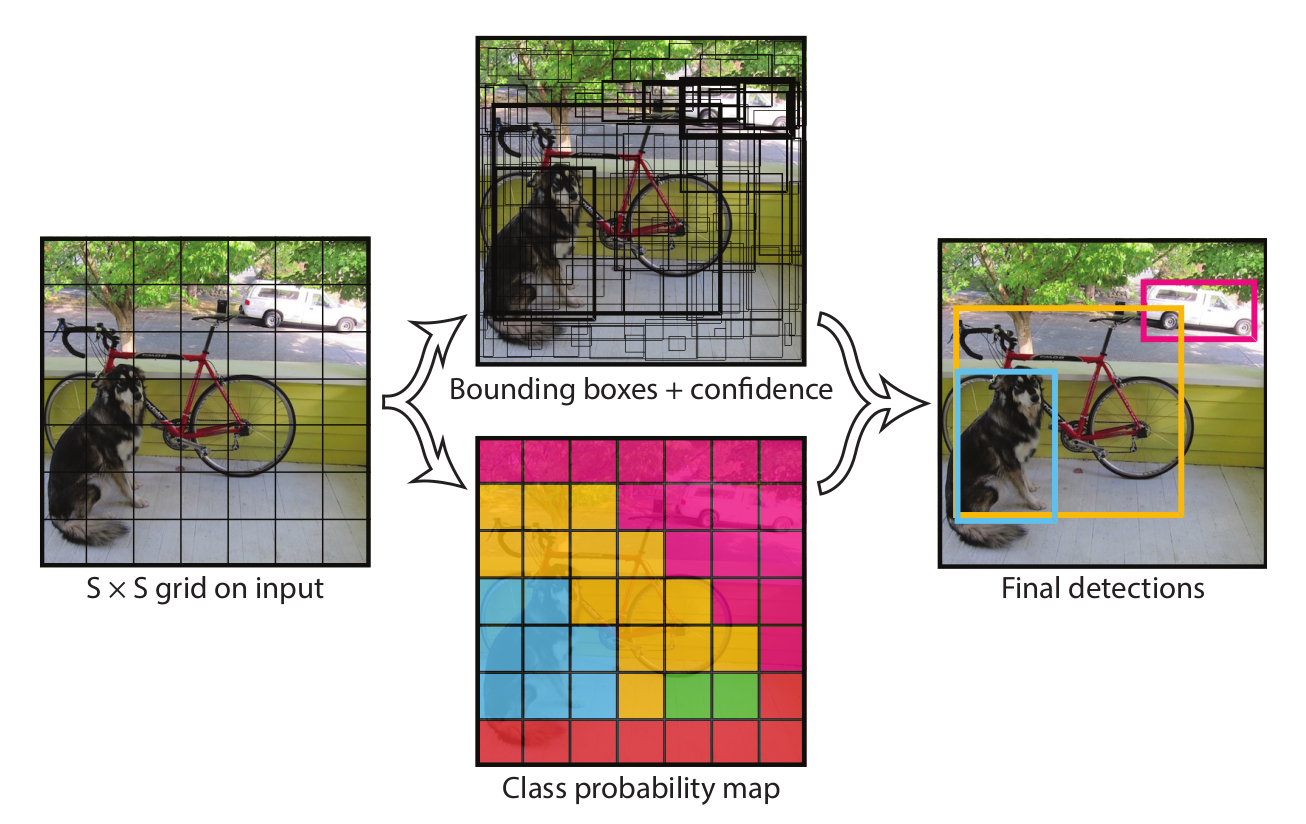
\includegraphics[width=0.85\textwidth]{images/yolo_v1_diagram.png}
    \caption{Detekce modelu (převzato z \cite{leimao_yolos_blog})}
    \label{fig:detection_principe}
\end{figure}

Na obrázku \ref{fig:detection_principe} je znázorněn způsob detekce objektů pomocí YOLO modelu, kde se rozděluje obraz do mřížky $S \times S$ a pro každou buňku mřížky predikuje B ohraničujících rámečků, spolehlivost pro tyto rámečky a pravděpodobnosti třídy C. Tyto predikce jsou kódovány ve formě tenzoru $S \times S \times (B \cdot 5 + C)$. 

\subsubsection{Klasifikace objektů}
Klasifikace objektů představuje úlohu přiřazení objektu do předem definované třídy
na základě jeho vizuálních charakteristik.
V oblasti dopravy je klasifikace využívána například pro rozlišení typů vozidel
nebo pro identifikaci specifických objektů v dopravním prostředí
\cite{szeliski_computer_vision}.

\subsubsection{Sledování objektů}
Sledování objektů umožňuje analyzovat pohyb detekovaných objektů napříč jednotlivými
snímky video sekvence.
Tato úloha je klíčová pro odhad trajektorií, rychlosti pohybu nebo hustoty dopravy.
Sledování objektů je často kombinováno s detekcí a klasifikací pro dosažení
komplexní analýzy dopravní situace \cite{zhou_traffic_survey_2024}.

\begin{figure}[H]
    \centering
    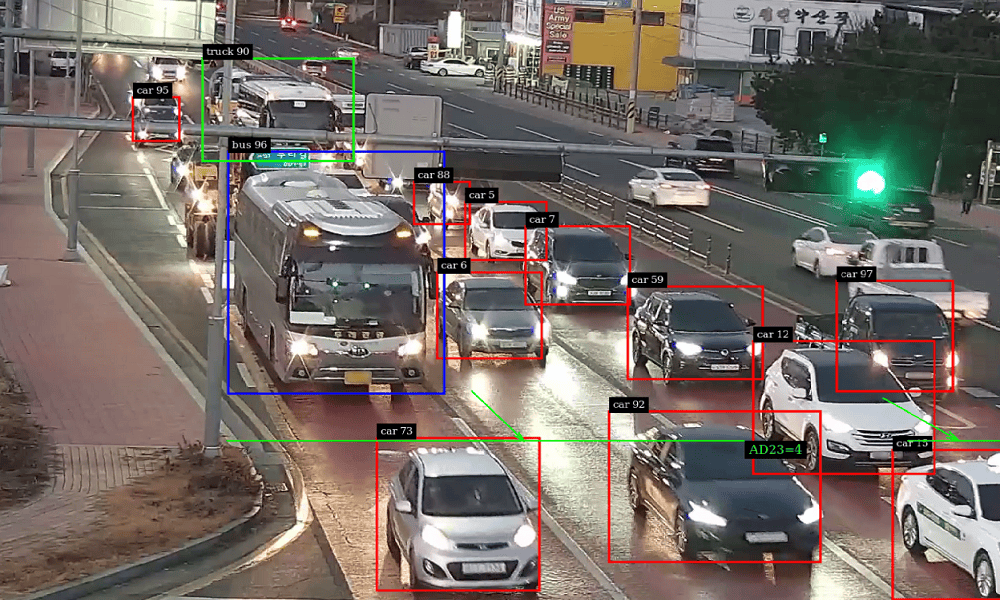
\includegraphics[width=0.9\textwidth]{images/object_tracking.png}
    \caption{Ukázka sledování objektů v dopravní scéně s přiřazenými identifikátory a třídami objektů \cite{augmentedstartups_traffic_tracking}}
    \label{fig:object_tracking_example}
\end{figure}

Sledování objektů představuje úlohu, jejímž cílem je udržení konzistentní identity
detekovaných objektů napříč jednotlivými snímky video sekvence.
Jak je znázorněno na obrázku~\ref{fig:object_tracking_example}, jednotlivým vozidlům
jsou přiřazeny unikátní identifikátory, které umožňují sledovat jejich pohyb v čase
a analyzovat jejich trajektorie.
Tento přístup je klíčový zejména v dopravních aplikacích, kde je nutné zabránit
vícenásobnému započítání téhož objektu.

\subsection{Předzpracování obrazu}
Předzpracování obrazu představuje důležitý krok před samotnou aplikací
detekčních a sledovacích algoritmů.
Cílem předzpracování je zlepšení kvality vstupních dat, redukce šumu
a optimalizace obrazových parametrů pro následné zpracování.

V dopravních aplikacích může být kvalita obrazu ovlivněna proměnlivými
světelnými podmínkami, povětrnostními vlivy nebo omezeným rozlišením
kamery. Proto je běžně využíváno škálování obrazu (resizing) na požadované
rozlišení vstupu detekčního modelu, normalizace pixelových hodnot a případné
omezení zpracovávané oblasti pomocí definice oblasti zájmu (ROI).

Redukce vstupního rozlišení může významně snížit výpočetní náročnost systému,
což je důležité zejména při nasazení na vestavěných zařízeních typu edge.
Současně však může docházet ke ztrátě detailů, což představuje kompromis
mezi rychlostí a přesností detekce \cite{szeliski_computer_vision}.


\subsection{Detekce objektů v reálném čase}
Detekce objektů v reálném čase klade důraz na rychlost zpracování a efektivní využití
výpočetních prostředků.
Tyto požadavky jsou zásadní zejména u vestavěných systémů a okrajových zařízení
(edge devices), která jsou často využívána v dopravní infrastruktuře.
Reálné nasazení zahrnuje například systémy pro rozpoznávání registračních značek
nebo sledování dopravy na křižovatkách \cite{hailo_alpr_2024}.

\subsection{Přehled detekčních modelů}
V posledních letech byly navrženy různé architektury hlubokých neuronových sítí pro
detekci objektů.
Mezi nejpoužívanější patří modely YOLO a SSD.
\subsubsection{Model YOLO}
Model YOLO (You Only Look Once) je jednofázový detekční model, který provádí detekci objektů v jediném průchodu neuronovou sítí.
Díky této vlastnosti dosahuje vysoké rychlosti zpracování, což jej činí vhodným pro aplikace v reálném čase, včetně dopravních systémů
\cite{redmon_yolo_2016}.

\begin{figure}[H]
    \centering
    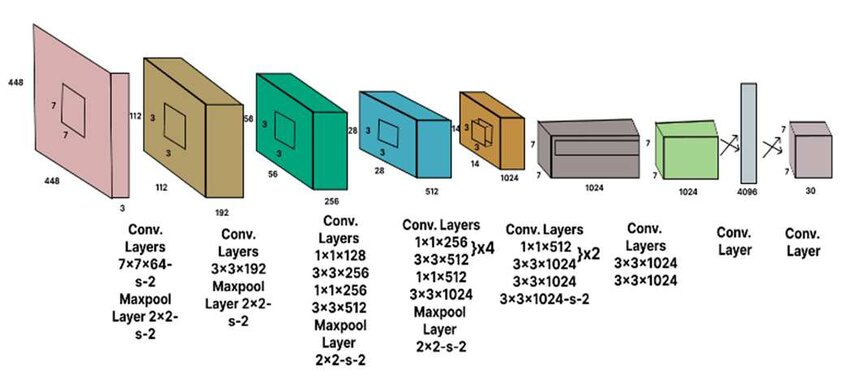
\includegraphics[width=0.85\textwidth]{images/yolo_model_conv.jpg}
    \caption{Architektura modelu YOLO (převzato z \cite{redmon_yolo_2016})}
    \label{fig:yolo_arch}
\end{figure}

Na obrázku \ref{fig:yolo_arch} je znázorněna architektura YOLO modelu, která má 24 konvolučních vrstev, po nichž následují 2 plně propojené vrstvy. Střídavé konvoluční vrstvy 1 × 1 zmenšují prostor pro prvky z předchozích vrstev. Konvoluční se předtrénují na klasifikační úloze ImageNet s polovičním rozlišením se vstupním obrázekem 224 × 224 px a poté zdvojnásobujeme rozlišení pro detekci.

\subsubsection{Srovnání vlastností modelů}
Při návrhu systému pro analýzu dopravy je nutné zohlednit kompromis mezi přesností
detekce a rychlostí zpracování.
Modely optimalizované na reálný čas jsou často preferovány v praktických
dopravních aplikacích, kde je kladen důraz na okamžitou odezvu systému
\cite{zhou_traffic_survey_2024}.


\section{Sledování a počítání objektů}
Sledování objektů v obraze a video sekvencích představuje klíčovou nadstavbu nad
detekcí objektů.
Zatímco detekce umožňuje lokalizovat objekty v jednotlivých snímcích, sledování
zajišťuje jejich konzistentní identifikaci napříč časem.
Tato vlastnost je zásadní zejména v dopravních aplikacích, kde je nutné analyzovat
pohyb vozidel, jejich trajektorie nebo počet průjezdů daným úsekem
\cite{szeliski_computer_vision, zhou_traffic_survey_2024}.

\subsection{Víceobjektové sledování (MOT)}
Víceobjektové sledování (Multiple Object Tracking, MOT) se zabývá současným
sledováním většího počtu objektů ve scéně.
Cílem je přiřazení konzistentních identifikátorů jednotlivým objektům a jejich
udržení po celou dobu jejich výskytu ve sledované sekvenci.
V dopravních systémech se víceobjektové sledování využívá například při analýze
dopravních toků, odhadu hustoty provozu nebo sledování pohybu vozidel na
křižovatkách \cite{zhou_traffic_survey_2024}.


Víceobjektové sledování je často realizováno kombinací detekce objektů a následného
přiřazování detekcí mezi jednotlivými snímky na základě prostorových a
časových charakteristik.

\begin{figure}[H]
    \centering
    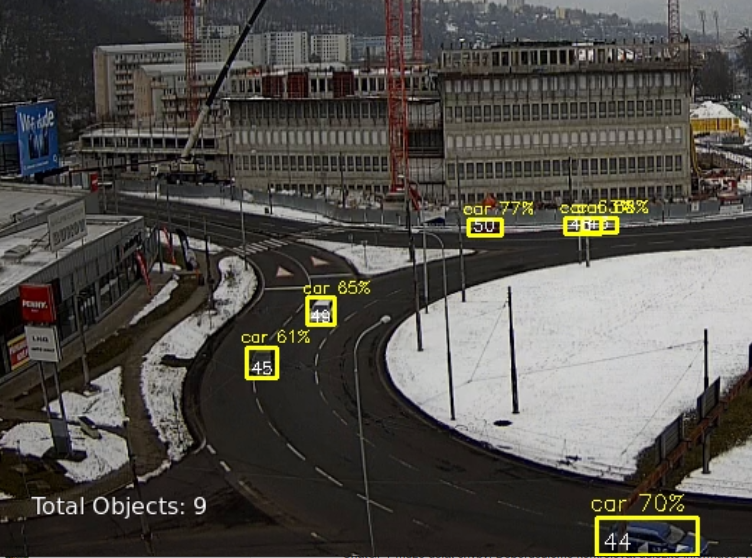
\includegraphics[width=0.9\textwidth]{images/own_tracking.png}
    \caption{Ukázka víceobjektového sledování vozidel s přiřazenými identifikátory (vlastní ilustrace)}
    \label{fig:own_tracking}
\end{figure}

Jak je patrné z obrázku \ref{fig:own_tracking}, navržený Hailo systém umožňující sledování (tracking)
více objektů najednou v reálném čase.

\subsection{Algoritmy pro sledování objektů}
Mezi nejpoužívanější přístupy pro sledování objektů v reálném čase patří algoritmy
SORT a DeepSORT.
Tyto metody jsou oblíbené zejména pro svou nízkou výpočetní náročnost a snadnou
integraci s detekčními modely, jako je YOLO \cite{redmon_yolo_2016}.

\subsubsection{SORT}
Algoritmus SORT (Simple Online and Realtime Tracking) je založen na kombinaci
Kalmanova filtru a algoritmu pro přiřazování objektů na základě minimální
vzdálenosti mezi detekcemi.
Každému sledovanému objektu je přiřazen unikátní identifikátor, který je udržován
v průběhu času.
Díky své jednoduchosti a rychlosti je SORT vhodný pro aplikace v reálném čase,
včetně dopravního dohledu \cite{SORT_original_2016}.

\begin{figure}[H]
    \centering
    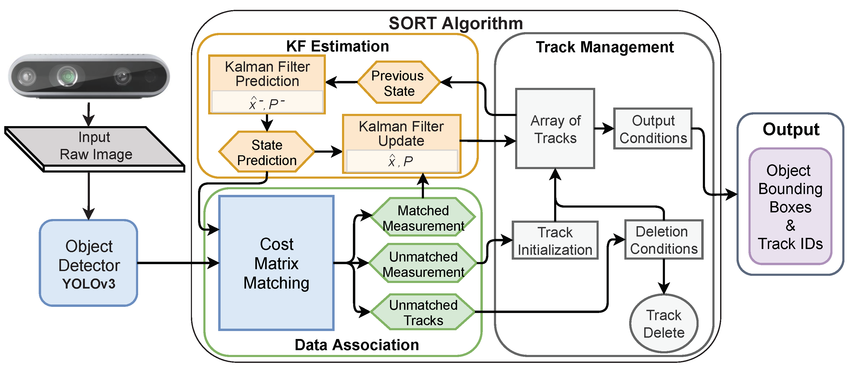
\includegraphics[width=0.9\textwidth]{images/sort_algoritm_principe.png}
    \caption{Overview of the object tracking SORT algorithm (adapted from \cite{SORT_original_2016})}
    \label{fig:sort_overview}
\end{figure}

Na obrázku ~\ref{fig:sort_overview} je znázorněno, jak SORT algoritmus kombinuje Kalmanovo filtrování s metodami přiřazování dat za účelem dosažení víceobjektového sledování v reálném čase \cite{SORT_original_2016}.

\subsubsection{DeepSORT}
DeepSORT rozšiřuje algoritmus SORT o využití hlubokých neuronových sítí pro extrakci
vzhledových příznaků sledovaných objektů.
Kromě prostorových informací tak bere v úvahu i vizuální podobnost objektů, což
výrazně zvyšuje robustnost sledování při častých překryvech nebo změnách pohybu.
Tento přístup je vhodný zejména v hustém dopravním provozu, kde dochází k častému
vzájemnému zakrývání objektů \cite{wojke_deepsort_2017}.

\begin{figure}[H]
    \centering
    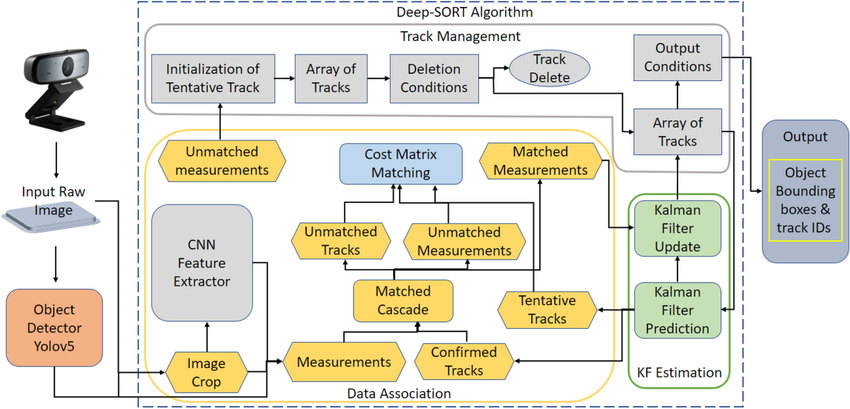
\includegraphics[width=0.9\textwidth]{images/deepsort_algoritm_principe.png}
    \caption{Přehled algoritmu DeepSORT a jeho rozhodovacích kroků (upraveno podle \cite{wojke_deepsort_2017})}
    \label{fig:deepsort_overview}
\end{figure}

Na obrázku \ref{fig:deepsort_overview} je znázorněn DeepSORT algoritmus, který rozšiřuje klasický tracking o vzhledový model založený na hlubokém
učení, což zlepšuje přiřazování identifikátorů při překrývání objektů
\cite{wojke_deepsort_2017}.

\subsubsection{Sledování objektů v systému Hailo}
Praktickým příkladem sledování objektů v reálném čase je řešení využívané v
platformě Hailo, která kombinuje detekci objektů s následným sledováním jejich
pohybu.
Systém využívá principy prostorového přiřazování detekcí mezi jednotlivými
snímky a správu identifikátorů objektů, což umožňuje sledovat objekty napříč
časem a analyzovat jejich trajektorie.
Tento přístup je využíván například v aplikacích automatického rozpoznávání
registračních značek a dopravního dohledu na okrajových zařízeních
\cite{hailo_alpr_2024}.

\subsubsection{Princip práce s identifikátory objektů}
Základním principem sledování objektů je přiřazení jednoznačného identifikátoru
(Unique ID) každému objektu při jeho prvním výskytu ve scéně.
Tento identifikátor je následně používán pro spojování detekcí mezi jednotlivými
snímky a umožňuje sledovat trajektorii objektu v čase.
Správná správa identifikátorů je klíčová pro následné úlohy, jako je počítání
objektů nebo analýza jejich pohybu \cite{szeliski_computer_vision, zhou_traffic_survey_2024}.

\subsection{Metody sčítání objektů}
Počítání objektů je často realizováno na základě výsledků víceobjektového
sledování.
Namísto jednoduchého počítání detekcí v jednotlivých snímcích se využívá informace
o trajektorii objektu, čímž se eliminuje riziko vícenásobného započítání téhož
objektu \cite{zhou_traffic_survey_2024}.

\subsubsection{Virtuální čára}
Jednou z nejpoužívanějších metod počítání objektů je využití virtuální čáry.
Objekt je započítán v okamžiku, kdy jeho trajektorie překročí předem definovanou
linii v obraze.
Tato metoda je vhodná například pro počítání průjezdů vozidel v konkrétním směru
a je široce využívána v dopravních monitorovacích systémech \cite{zhou_traffic_survey_2024}.

\subsubsection{Oblast zájmu (ROI)}
Alternativním přístupem je definice oblasti zájmu (Region of Interest, ROI), ve
které jsou objekty sledovány a započítávány.
Objekt je započítán při vstupu do dané oblasti nebo při jejím opuštění.
Tento přístup je vhodný zejména pro analýzu obsazenosti parkovacích míst nebo
sledování pohybu vozidel v konkrétním prostoru \cite{szeliski_computer_vision, zhou_traffic_survey_2024}.

\begin{figure}[H]
    \centering
    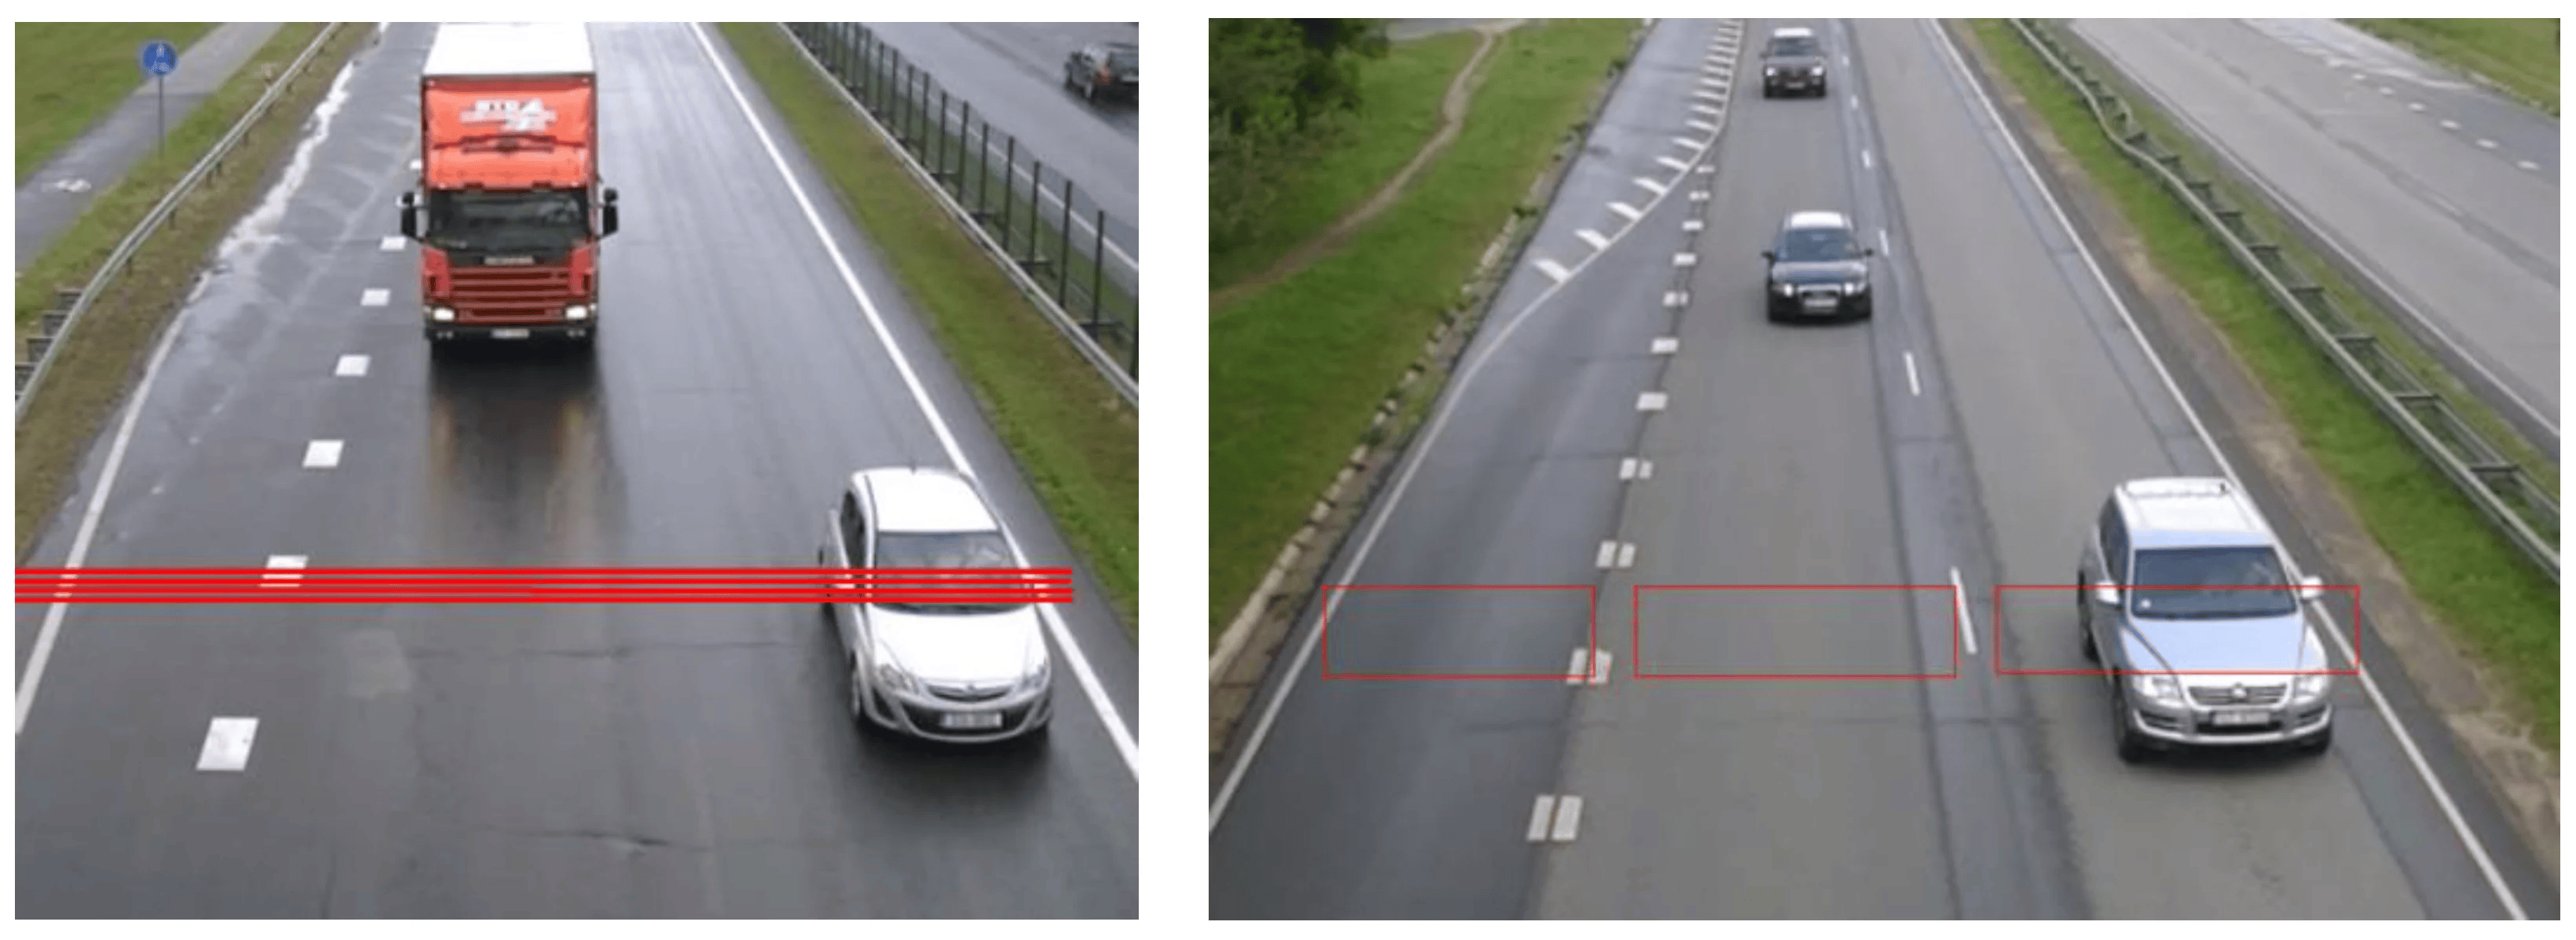
\includegraphics[width=0.85\textwidth]{images/roi_line.png}
    \caption{Detekce objektů z ROI oblasti pomocí virtuální čáry (upraveno podle \cite{mdpi_roi_tracking_2022})}
    \label{fig:roi_line}
\end{figure}

Obrázek \ref{fig:roi_line} znázorňuje princip detekce a sčítání objektů
využívající oblast zájmu (Region of Interest, ROI) a virtuální detekční čáru.
ROI představuje vybranou část obrazu, ve které je prováděna analýza pohybujících
se objektů, čímž dochází ke snížení výpočetní náročnosti zpracování obrazu.
Virtuální čára je umístěna kolmo na směr pohybu sledovaných objektů a slouží
jako referenční hranice pro jejich započítání.

Objekt je detekován a započítán v okamžiku, kdy jeho trajektorie protne
virtuální čáru. Tento přístup umožňuje určit nejen počet objektů, ale také
směr jejich pohybu. Metoda je často využívána v dopravních monitorovacích
systémech, kde umožňuje efektivní sledování vozidel nebo chodců při zachování
nízkých výpočetních nároků \cite{mdpi_roi_tracking_2022}.

\section{Systémy pro monitorování dopravy}
Monitorování dopravy představuje klíčovou součást moderních inteligentních
dopravních systémů.
Jeho cílem je získávání informací o dopravním provozu, jako je intenzita dopravy,
rychlost vozidel nebo výskyt dopravních událostí.
Tyto informace jsou následně využívány pro řízení dopravy, plánování infrastruktury
a zvyšování bezpečnosti silničního provozu \cite{zhou_traffic_survey_2024}.

\subsection{Tradiční metody dopravního monitoringu}
Tradiční metody monitorování dopravy jsou založeny převážně na fyzických senzorech
nebo manuálním sběru dat.
Mezi jejich hlavní výhody patří relativně jednoduchá implementace a dlouhodobé
využívání v praxi, nevýhodou je však omezená flexibilita a vysoké náklady na údržbu.

Jednou z nejstarších metod je manuální sčítání dopravy, při kterém jsou dopravní
prostředky zaznamenávány lidským pozorovatelem.
Tento přístup je časově náročný, náchylný k chybám a nevhodný pro dlouhodobý
monitoring dopravního provozu \cite{zhou_traffic_survey_2024}.

Další rozšířenou technologií jsou indukční smyčky zabudované do vozovky, které
detekují přítomnost vozidla na základě změny elektromagnetického pole.
Ačkoliv poskytují relativně přesná data o průjezdech vozidel, jejich instalace
vyžaduje zásah do vozovky a pravidelnou údržbu \cite{zhou_traffic_survey_2024}.

Pro monitorování dopravy jsou rovněž využívány radarové a lidarové senzory, které
umožňují měření vzdálenosti a rychlosti objektů.
Tyto technologie dosahují vysoké přesnosti, avšak jejich nevýhodou jsou vyšší
pořizovací náklady a omezené možnosti rozlišení jednotlivých typů objektů
\cite{zhou_traffic_survey_2024}.

\subsection{Moderní kamerové systémy}
S rozvojem počítačového vidění a výpočetního výkonu se stále častěji prosazují
kamerové systémy založené na analýze obrazových dat.
Kamerové systémy umožňují získávat bohaté informace o dopravní scéně, včetně typu
vozidel, jejich trajektorií nebo chování účastníků provozu
\cite{szeliski_computer_vision}.

Mezi hlavní výhody kamerových systémů patří jejich vysoká flexibilita, možnost
softwarových úprav a využití jednoho zařízení pro více analytických úloh.
Moderní přístupy založené na hlubokém učení umožňují detekci a sledování objektů v
reálném čase, což je klíčové pro nasazení v inteligentních dopravních systémech
\cite{redmon_yolo_2016, zhou_traffic_survey_2024}.

Nevýhodou kamerových systémů jsou jejich limity spojené s kvalitou vstupních dat.
Výkon detekčních a sledovacích algoritmů může být ovlivněn změnami světelných
podmínek, nepříznivým počasím nebo vzájemným překrýváním objektů ve scéně.
Tyto faktory představují výzvu zejména v hustém městském provozu
\cite{zhou_traffic_survey_2024}.

\begin{figure}[H]
    \centering
    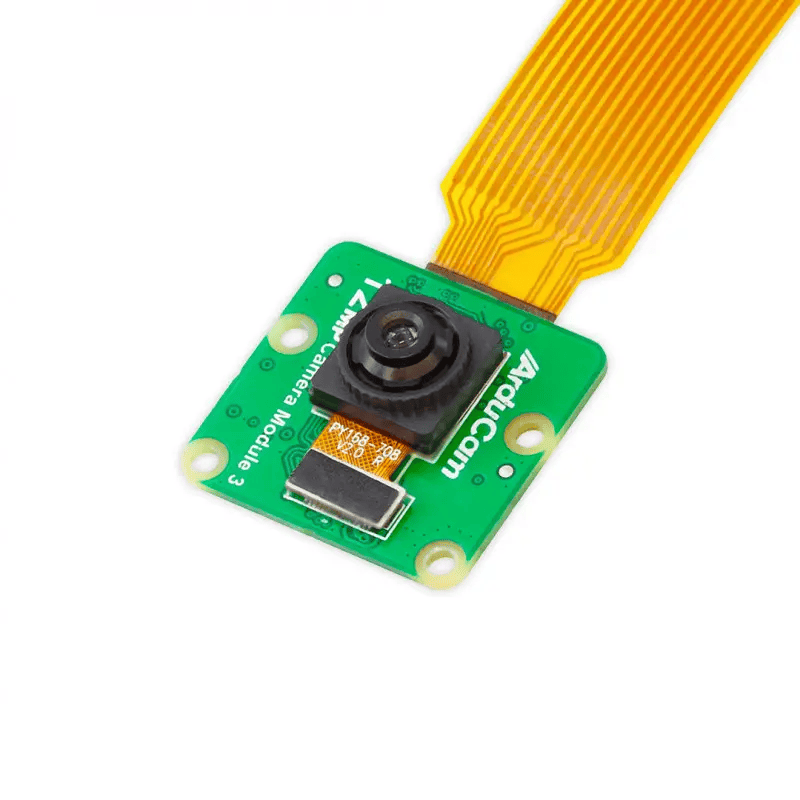
\includegraphics[width=0.7\textwidth]{images/AI_camera.png}
    \caption{Kamerový modul Arducam IMX708 určený pro platformu Raspberry Pi \cite{rpishop_imx708}}
    \label{fig:ai_camera}
\end{figure}

Na obrázku \ref{fig:ai_camera} je znázorněn speciální kamerový modul Arducam IMX708 určený
pro platformu Raspberry Pi. Kamera je vybavena obrazovým snímačem Sony IMX708
s rozlišením přibližně 12 megapixelů, který umožňuje pořizování snímků a videa
ve vysoké kvalitě. Modul využívá objektiv s pevným zaostřením, což přispívá k
rychlé odezvě při snímání a stabilní kvalitě obrazu bez nutnosti mechanického
přeostřování.

Kamera podporuje více režimů rozlišení, které umožňují optimalizovat poměr mezi
kvalitou obrazu a výpočetní náročností zpracování. Díky podpoře HDR režimu je
možné zachytit scénu s vyšším dynamickým rozsahem, což zlepšuje detekci objektů
v proměnlivých světelných podmínkách. Tyto vlastnosti činí modul vhodným pro
aplikace počítačového vidění a edge AI systémy využívané například při monitorování
dopravních situací.

\subsection{Existující řešení a projekty}
přehled dostupných systémů
srovnání s navrhovaným řešením

V současnosti existuje řada komerčních i výzkumných řešení zaměřených na monitorování
dopravy pomocí kamerových systémů.
Tato řešení často kombinují detekci objektů, sledování pohybu a následnou analýzu dopravních dat.

Příkladem praktického nasazení kamerových systémů je automatické rozpoznávání
registračních značek, které nachází uplatnění při dohledu nad dopravou nebo
kontrole přístupu \cite{hailo_alpr_2024}.
Moderní systémy jsou stále častěji implementovány na okrajových
zařízeních (edge devices), kde je kladen důraz na nízkou latenci,
efektivní využití výpočetních prostředků a minimalizaci přenosu
velkého objemu dat do cloudové infrastruktury
\cite{li_edge_ai_2020}.


Navrhované řešení v rámci této práce se od existujících systémů odlišuje důrazem na
modularitu, využití otevřených technologií a možnost přizpůsobení konkrétním
podmínkám monitorovaného prostředí.

\section{Edge AI a vestavěné systémy}
Edge AI označuje přístup, při kterém jsou úlohy umělé inteligence
realizovány přímo na okrajových zařízeních v blízkosti zdroje dat,
nikoliv v centrálním cloudovém prostředí.
Tento koncept umožňuje snížení latence, omezení přenosu dat
a efektivnější využití síťových zdrojů
\cite{li_edge_ai_2020}.

\subsection{Zpracování obrazu na okraji sítě}
Zpracování obrazu na okraji sítě představuje alternativu ke klasickému cloudovému
zpracování, kdy jsou obrazová data přenášena do vzdáleného datového centra.
V případě edge přístupu jsou data analyzována přímo na zařízení, které obraz
získává, což výrazně snižuje přenosové nároky a zvyšuje odezvu systému.

Hlavním rozdílem mezi edge a cloudovým přístupem je latence
a nároky na přenos dat.
Zatímco cloudové řešení vyžaduje odesílání obrazových dat
do vzdálených datových center, edge řešení umožňuje
lokální inferenci neuronových sítí přímo na zařízení,
čímž se minimalizuje zpoždění a zvyšuje robustnost systému
\cite{li_edge_ai_2020}.

\begin{figure}[H]
    \centering
    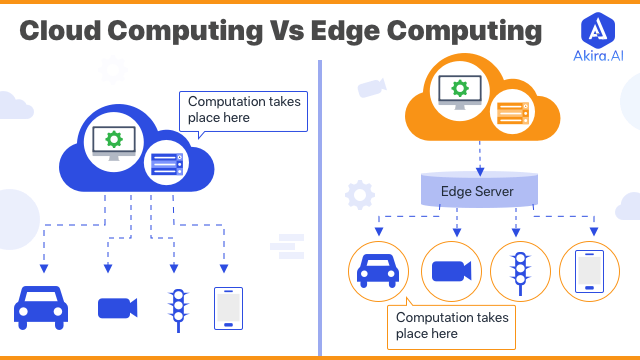
\includegraphics[width=0.9\textwidth]{images/akira-ai-cloud-computing-vs-edge-computing.png}
    \caption{Srovnání edge a cloudového zpracování obrazových dat \cite{akira_edge_cloud}}
    \label{fig:edge_vs_cloud}
\end{figure}

Na obrázku je znázorněno porovnání architektury cloud computingu a edge
computingu. Cloud computing využívá centralizovaná datová centra pro
zpracování dat, zatímco edge computing provádí výpočty přímo v blízkosti
zdroje dat, což umožňuje rychlejší odezvu systému a nižší latenci
\cite{akira_edge_cloud}.


\subsection{AI akcelerátory}
AI akcelerátory jsou specializovaná hardwarová zařízení navržená pro efektivní
provádění výpočtů spojených s umělými neuronovými sítěmi.
Na rozdíl od univerzálních procesorů jsou optimalizovány pro paralelní zpracování
operací, které jsou typické pro inferenci hlubokých modelů.

V kontextu edge AI nacházejí akcelerátory uplatnění zejména při zpracování obrazu v
reálném čase, kde je kladen důraz na vysoký výkon při omezené spotřebě energie.
Použití akcelerátorů umožňuje nasazení pokročilých detekčních a sledovacích modelů
i na energeticky úsporných vestavěných zařízeních \cite{hailo_alpr_2024}.

Díky akcelerátorům je možné realizovat komplexní analytické úlohy, jako je detekce,
sledování a počítání objektů, přímo na okrajových zařízeních bez nutnosti využití
výkonných serverových systémů.

\subsection{Platforma Raspberry Pi}
vlastnosti, omezení, vhodnost pro daný úkol

Platforma Raspberry Pi představuje rozšířenou rodinu jednodeskových počítačů, které
jsou často využívány pro prototypování a vývoj vestavěných systémů.
Díky nízké pořizovací ceně, široké komunitní podpoře a dostupnosti rozšiřujících
modulů je Raspberry Pi vhodným nástrojem pro experimentální i aplikační využití
\cite{raspberrypi_docs_2024}.

Mezi hlavní vlastnosti platformy Raspberry Pi patří kompaktní rozměry, nízká spotřeba
energie a podpora různých operačních systémů.
Tyto vlastnosti umožňují jeho nasazení v distribuovaných systémech monitorování
dopravy, zejména v kombinaci s externími akcelerátory pro zpracování umělé
inteligence \cite{raspberrypi_ai_kit}.

Omezením platformy Raspberry Pi je relativně omezený výpočetní výkon ve srovnání s
výkonnými desktopovými nebo serverovými systémy.
Z tohoto důvodu není vhodná pro trénování hlubokých neuronových sítí, avšak v
kombinaci s AI akcelerátory představuje efektivní řešení pro inferenci modelů v
reálném čase, což odpovídá požadavkům řešeného úkolu.

\begin{figure}[H]
    \centering
    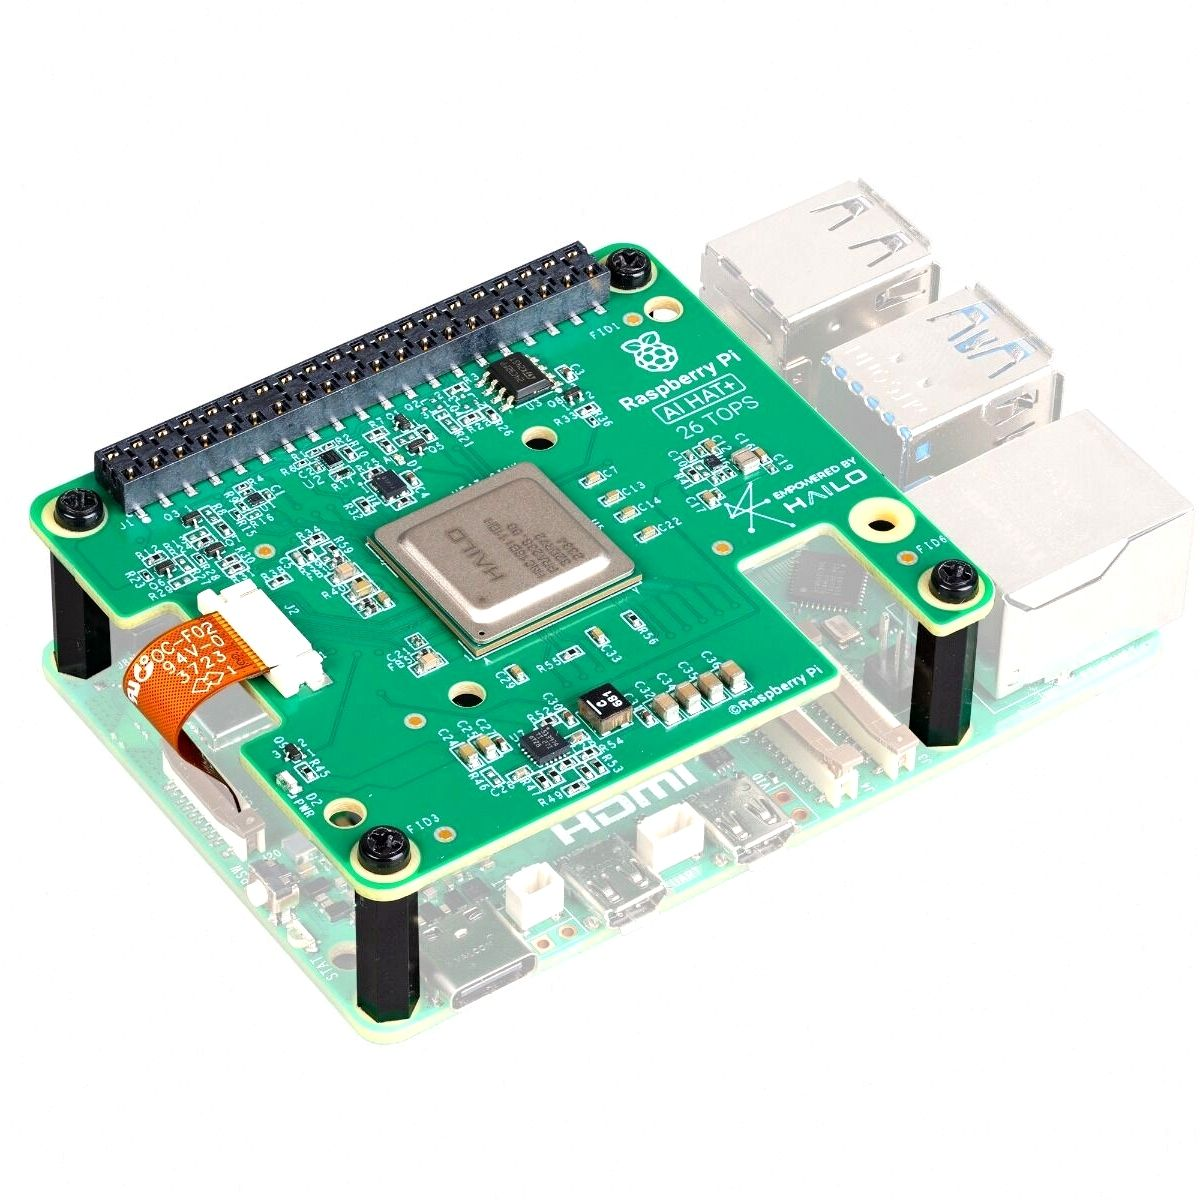
\includegraphics[width=0.75\textwidth]{images/device_with_hailo_processor.jpg}
    \caption{Raspberry Pi AI HAT+ TOPS 26 (Rpishop)}
    \label{fig:hailo_antratek}
\end{figure}

Na obrázku \ref{fig:hailo_antratek} je zobrazen modul Raspberry Pi AI HAT+, který představuje vysoce výkonné řešení pro akceleraci úloh umělé inteligence na platformě Raspberry Pi 5. Hlavním prvkem této rozšiřující desky je integrovaný AI procesor Hailo-8 od společnosti Hailo Technologies. Klíčovým parametrem tohoto zařízení je výpočetní výkon dosahující 26 TOPS (Tera Operations Per Second), což značí schopnost procesoru vykonat 26 bilionů operací za sekundu při inferenci hlubokých neuronových sítí.

Díky této vysoké propustnosti a architektuře optimalizované pro nízkou spotřebu energie umožňuje modul plynulé zpracování komplexních modelů, jako je YOLO, v reálném čase přímo na okrajovém zařízení. V kombinaci s rozhraním PCIe, které zajišťuje rychlý přenos dat mezi procesorem a kamerovým modulem, tvoří toto řešení ideální základ pro systémy monitorování dopravy, kde je vyžadována nízká latence a vysoká přesnost detekce bez závislosti na cloudových službách.

\section{Metodika testování a evaluace}
Vyhodnocení kvality systémů pro detekci, sledování a počítání objektů představuje
nedílnou součást návrhu a implementace řešení založených na počítačovém vidění.
Cílem evaluace je objektivně posoudit přesnost a spolehlivost navrženého systému a
identifikovat jeho silné a slabé stránky.
V oblasti dopravního monitorování je důležité hodnotit nejen přesnost detekce,
ale také správnost následného sčítání objektů \cite{szeliski_computer_vision, zhou_traffic_survey_2024}.

\subsection{Metriky hodnocení detekce}
Pro hodnocení kvality detekce objektů se běžně využívají metriky založené na porovnání
výstupů detekčního systému s referenčními daty, označovanými jako ground truth.
Tyto metriky umožňují kvantifikovat schopnost systému správně identifikovat objekty
a minimalizovat chybné detekce \cite{szeliski_computer_vision}.

\subsubsection{Precision}
Metrika precision vyjadřuje podíl správně detekovaných objektů
(True Positives) vzhledem k celkovému počtu detekcí provedených systémem,
tedy součtu správných a falešně pozitivních detekcí:

$$
Precision = \frac{TP}{TP + FP}.
$$

Tato metrika je součástí standardního vyhodnocení detekčních modelů
v rámci benchmarku Pascal VOC \cite{everingham2010voc}.

\subsubsection{Recall}
Metrika recall udává schopnost systému nalézt všechny relevantní objekty
přítomné ve scéně. Je definována jako podíl správně detekovaných objektů
vzhledem k celkovému počtu objektů v referenčních datech:

$$
Recall = \frac{TP}{TP + FN}.
$$

Recall je společně s precision základní složkou
Precision–Recall křivky používané při výpočtu AP a mAP
\cite{everingham2010voc}.

\subsubsection{IoU (Intersection over Union)}
Metrika IoU (Intersection over Union) vyjadřuje míru překryvu mezi
predikovaným ohraničujícím rámečkem $B_p$ a referenčním rámečkem
$B_{gt}$ (ground truth). Je definována jako podíl plochy jejich průniku
a plochy jejich sjednocení:
$$IoU = \frac{area(B_p \cap B_{gt})}{area(B_p \cup B_{gt})}$$
V rámci benchmarku Pascal VOC je detekce považována za správnou,
pokud $IoU \geq 0{,}5$ \cite{everingham2010voc}.

\subsubsection{Average Precision (AP)}

Average Precision (AP) je definována jako plocha pod křivkou
precision–recall (PR křivka).
Tato metrika zohledňuje jak přesnost (precision), tak úplnost (recall)
v různých prahových hodnotách detekční jistoty.

V rámci Pascal VOC Challenge je AP počítána pro každou třídu
samostatně na základě porovnání detekcí s referenčními anotacemi
\cite{everingham2010voc}.

\subsubsection{Mean Average Precision (mAP)}
Mean Average Precision (mAP) představuje aritmetický průměr hodnot AP
napříč všemi třídami objektů. Tato metrika je standardním ukazatelem
výkonu detekčních modelů v benchmarkových úlohách objektové detekce
\cite{everingham2010voc}.

mAP poskytuje komplexní informaci o kvalitě modelu, neboť zohledňuje
jak schopnost správné lokalizace objektů (IoU), tak jejich správnou
klasifikaci.

\subsubsection{Accuracy}
Metrika accuracy vyjadřuje celkový podíl správných rozhodnutí systému.
V kontextu detekce objektů je její interpretace omezená, zejména v případech, kdy
dochází k výrazné nerovnováze mezi počtem objektů a pozadím.
Z tohoto důvodu se metrika accuracy u objektové detekce obvykle nepovažuje
za primární hodnoticí ukazatel a její použití je omezené.\cite{szeliski_computer_vision}.

\subsection{Metodika vyhodnocení systému}
Vzhledem k povaze práce je vyhodnocení systému rozděleno do dvou fází, které se liší dostupností referenčních dat a způsobem výpočtu přesnosti.

\subsubsection{Evaluace s využitím referenčního datasetu}
Při testování na anotovaných datech (např. veřejné dopravní datasety) jsou využívány exaktní metriky mAP a IoU. Tento přístup umožňuje přesné srovnání různých verzí detekčních modelů v kontrolovaných podmínkách \cite{zhou_traffic_survey_2024}.

\subsubsection{Evaluace systému v reálném prostředí (bez datasetu)}
V reálném nasazení, kde nejsou k dispozici předem připravené anotace, je využívána metoda srovnání s manuálním sčítáním \cite{mdpi_roi_tracking_2022}.
Referenční hodnota je získána manuálním pozorováním videozáznamu, kdy je zaznamenán skutečný počet vozidel ($N_{real}$). Ten je následně porovnán s počtem vozidel detekovaným systémem ($N_{sys}$):
$$Accuracy_{count} = 1 - \frac{|N_{real} - N_{sys}|}{N_{real}}$$
Tato metrika reflektuje celkovou úspěšnost systému při sčítání vozidel v reálném čase.

Vzhledem k tomu, že v práci je využíván předtrénovaný model YOLO,
není cílem optimalizace samotného modelu, ale ověření jeho
výkonu v konkrétním dopravním prostředí.

\subsubsection{Vyhodnocení sčítání objektů}
Vyhodnocení správnosti sčítání objektů je v dopravních aplikacích klíčové, neboť
výsledné počty vozidel často slouží jako podklad pro další analýzy a rozhodování.
Na rozdíl od detekce jednotlivých snímků se zde hodnotí konzistence sledování objektů
v čase a správná identifikace jejich průchodů definovanými oblastmi.

Jedním z běžně používaných přístupů je porovnání automaticky získaných výsledků s
manuálním pozorováním.
Manuální sčítání slouží jako referenční metoda, vůči které je možné vyhodnotit
odchylku a chybu automatického systému \cite{zhou_traffic_survey_2024}.

Mezi hlavní zdroje chyb při sčítání objektů patří zejména chybné přiřazení
identifikátorů objektů, ztráta sledovaného objektu při překrytí nebo opakované
započítání téhož objektu.
Tyto chyby jsou často způsobeny nepříznivými podmínkami snímání, jako je hustý provoz,
proměnlivé osvětlení nebo omezená kvalita vstupního obrazu.

\section{Etické aspekty a GDPR}
Při nasazení kamerových systémů v dopravě je nutné zohlednit
ochranu osobních údajů a principy vyplývající z Nařízení
Evropského parlamentu a Rady (EU) 2016/679 (GDPR).
Navržené řešení respektuje princip \textit{privacy by design},
tedy ochranu soukromí již ve fázi návrhu systému.
Zpracování obrazových dat probíhá přímo na okrajovém zařízení
(edge device), čímž se minimalizuje přenos surových dat do
externí infrastruktury a snižuje riziko jejich zneužití
\cite{li_edge_ai_2020}. Do databáze jsou ukládána pouze anonymizovaná metadata
o průjezdech vozidel (např. čas a směr pohybu),
nikoliv samotná obrazová data.
Tento přístup odpovídá zásadě minimalizace údajů,
která je jedním ze základních principů GDPR.


\chapter{Návrh systému}
\section{Požadavky na systém}
Navrhovaný systém je určen pro automatizovanou analýzu silniční dopravy 
pomocí metod počítačového vidění. Cílem je detekce a sledování vozidel 
v reálném čase a následná extrakce statistických údajů o jejich průjezdech.

Mezi hlavní funkční požadavky patří:

\begin{itemize}
    \item detekce vozidel v obrazové sekvenci,
    \item sledování objektů napříč jednotlivými snímky,
    \item identifikace průjezdu definovanou detekční linií (ROI),
    \item ukládání detekčních událostí do databáze,
    \item vizualizace agregovaných statistik.
\end{itemize}

Systém musí být schopen provozu v reálném čase na vestavěném zařízení 
s omezenými výpočetními prostředky. Z tohoto důvodu je navržena 
architektura založená na principu edge computing, kdy je inference 
neuronové sítě prováděna přímo na zařízení v místě sběru dat 
\cite{akira_edge_cloud}.

\subsection{Logika detekční linie (ROI)}
Pro účely počítání vozidel je v obraze definována virtuální detekční linie,
která představuje referenční hranici pro započítání průjezdu.
Každému sledovanému objektu je přiřazen unikátní identifikátor (ID),
který je udržován v průběhu jeho výskytu ve scéně.

Průjezd je zaznamenán v okamžiku, kdy střed ohraničujícího rámečku
sledovaného objektu překročí definovanou linii.
Aby nedocházelo k vícenásobnému započítání téhož objektu,
je každé ID započítáno pouze jednou při prvním překročení linie.

Systém rovněž umožňuje rozlišení směru pohybu na základě
porovnání předchozí a aktuální polohy objektu vůči detekční linii.
Tato logika umožňuje evidovat samostatně příjezdy a odjezdy vozidel.


\section{Celková architektura řešení}
\subsection{Přehled architektury}
Architektura systému je navržena jako vícevrstvá a modulární. 
Jednotlivé komponenty jsou odděleny podle své funkce, což umožňuje 
lepší škálovatelnost, robustnost a údržbu systému.

Systém se skládá z následujících vrstev:

\begin{enumerate}
    \item Vrstva akvizice obrazu,
    \item Vrstva zpracování videa (detekce a tracking),
    \item Komunikační vrstva,
    \item Datová vrstva,
    \item Aplikační a vizualizační vrstva.
\end{enumerate}

Takto strukturovaný přístup odpovídá moderním architekturám 
dopravních monitorovacích systémů založených na počítačovém vidění 
\cite{zhou_traffic_survey_2024}.

\subsection{Tok dat v systému}
Tok dat systémem je navržen následovně:

\begin{enumerate}
    \item IP kamera poskytuje kontinuální video stream.
    \item Obrazová data jsou předzpracována a předána detekčnímu modelu.
    \item Model provádí lokalizaci objektů pomocí metody typu YOLO 
    \cite{redmon_yolo_2016, leimao_yolos_blog}.
    \item Sledovací algoritmus přiřazuje jednotlivým objektům unikátní identifikátory 
    (např. na principu algoritmu SORT \cite{SORT_original_2016}).
    \item Je vyhodnocen průchod objektu přes virtuální detekční linii 
    \cite{mdpi_roi_tracking_2022}.
    \item Strukturované detekční události jsou odeslány do datové vrstvy.
    \item Aplikační vrstva poskytuje statistické přehledy uživateli.
\end{enumerate}

Oddělení jednotlivých kroků umožňuje modularitu systému 
a minimalizaci vzájemné závislosti komponent.

\section{Výběr hardwaru}

\subsection{Kamerový systém}
Pro zajištění dostatečné kvality detekce je využita IP kamera značky
Hikvision, která umožňuje síťový přenos video streamu prostřednictvím
protokolů RTSP nebo HTTP.
Použití IP kamery umožňuje flexibilní umístění zařízení mimo samotný
výpočetní uzel a současně poskytuje vyšší odolnost vůči povětrnostním
podmínkám v porovnání s běžnými kamerovými moduly pro vestavěná zařízení.

IP kamera poskytuje video stream ve vysokém rozlišení, což je důležité pro přesnou detekci vozidel zejména ve větší vzdálenosti od kamery.
Zpracování obrazu je následně prováděno na edge zařízení, které přijímá datový tok prostřednictvím lokální sítě.

\subsection{Zpracovatelská jednotka}
Jako výpočetní platforma je navrženo zařízení Raspberry Pi, 
které představuje vhodný kompromis mezi výkonem, spotřebou 
a cenou \cite{raspberrypi_docs_2024}.

Pro zajištění real-time inference neuronové sítě je navržen 
dedikovaný AI akcelerátor kompatibilní s touto platformou 
\cite{raspberrypi_ai_kit}. Tento přístup umožňuje efektivní 
zpracování obrazu na hraně sítě bez nutnosti využití cloudových služeb.

\section{Návrh softwarové architektury}
Softwarová architektura je navržena jako distribuovaná 
a asynchronní. Jednotlivé komponenty komunikují prostřednictvím 
lehkého zprávového protokolu MQTT \cite{mqtt_oasis_2019}.

\subsection{Detekční a sledovací modul}
Detekční modul je založen na konvoluční neuronové síti typu YOLO, 
která umožňuje rychlou lokalizaci objektů v obraze 
\cite{redmon_yolo_2016}. Pro sledování objektů napříč snímky 
je navržen algoritmus typu SORT \cite{SORT_original_2016} 
nebo jeho rozšířená varianta DeepSORT \cite{wojke_deepsort_2017}.

\subsection{Modul pro ukládání dat}
Detekční události jsou ukládány do relační databáze PostgreSQL, 
která umožňuje strukturované ukládání dat a jejich následné 
statistické vyhodnocení \cite{psycopg_docs_2025}. 
Pro numerické a statistické operace je možné využít knihovny 
NumPy \cite{harris_numpy_2020} a Pandas \cite{mckinney_pandas_2010}.

\subsubsection{Návrh databáze}

\subsection{Vizualizační modul}
Vizualizace dat je navržena formou webového rozhraní s využitím 
interaktivních grafů. Pro tvorbu grafických výstupů lze využít 
knihovnu Plotly \cite{plotly_docs_2015}, která umožňuje 
zobrazení časových řad, histogramů a agregovaných statistik.

\subsection{Architektonické schéma systému}

\begin{figure}[H]
    \centering
    \includegraphics[width=\textwidth]{images/architecture.png}
    \caption{Navržená architektura systému pro analýzu dopravy}
    \label{fig:architektura}
\end{figure}

Na Obr.~\ref{fig:architektura} je znázorněna navržená architektura systému.
Diagram zachycuje rozdělení systému do jednotlivých vrstev a tok dat mezi nimi.

Architektura systému je rozdělena do čtyř hlavních částí:

\begin{itemize}
    \item Síťová vrstva – zajišťuje přenos video streamu z IP kamery.
    \item Edge vrstva – provádí real-time detekci objektů pomocí AI modulu.
    \item Komunikační vrstva – realizovaná pomocí MQTT brokeru \cite{mqtt_oasis_2019}.
    \item Backendová vrstva – zajišťuje ukládání dat a poskytování API rozhraní.
\end{itemize}

Video stream je přenášen pomocí protokolu RTSP do edge zařízení, kde probíhá
detekce objektů pomocí neuronové sítě typu YOLO \cite{redmon_yolo_2016}.
Výsledné detekční události jsou odesílány prostřednictvím MQTT
a následně ukládány do databáze.

Frontendová vrstva komunikuje s backendem pomocí REST API
a umožňuje vizualizaci agregovaných statistik.


\chapter{Implementace systému}

\begin{table}[H]
\centering
\begin{tabular}{|l|l|}
\hline
Komponenta & Použitá technologie \\
\hline
Operační systém & Raspberry Pi OS \\
Programovací jazyk & Python 3.11 \\
AI inference & HailoRT + TAPPAS \\
Zpracování videa & GStreamer \\
Komunikace & MQTT \\
Databáze & PostgreSQL \\
API & FastAPI \\
Vizualizace & Streamlit + Plotly \\
\hline
\end{tabular}
\caption{Použité technologie v implementaci systému}
\end{table}

\section{Příprava vývojového prostředí}
Pro implementaci navrženého systému bylo nutné připravit 
vývojové prostředí odpovídající cílové hardwarové platformě 
a požadavkům na real-time zpracování obrazu.

\subsection{Operační systém}

Cílovou platformou systému je zařízení Raspberry Pi 5.
Na zařízení byl nainstalován operační systém Raspberry Pi OS 
založený na distribuci Debian Linux \cite{raspberrypi_docs_2024}.

Tento operační systém byl zvolen z důvodu:

\begin{itemize}
    \item plné podpory hardwaru Raspberry Pi,
    \item kompatibility s AI akcelerátorem,
    \item dostupnosti potřebných knihoven pro práci s obrazem a sítí,
    \item dlouhodobé podpory a aktualizací.
\end{itemize}

Systém byl konfigurován pro automatické spuštění detekční služby 
po startu zařízení.

\subsection{Programovací jazyk a základní knihovny}

Implementace systému byla realizována v programovacím jazyce Python 
ve verzi 3.11 \cite{python_docs_313_2025}. 

Python byl zvolen zejména díky:

\begin{itemize}
    \item široké podpoře knihoven pro počítačové vidění,
    \item jednoduché integraci s databázovými systémy,
    \item dostupnosti frameworků pro tvorbu webového API.
\end{itemize}

Pro numerické operace a práci s datovými strukturami byly využity knihovny:

\begin{itemize}
    \item NumPy \cite{harris_numpy_2020},
    \item Pandas \cite{mckinney_pandas_2010}.
\end{itemize}

\subsection{Framework pro zpracování videa a inference}

Pro real-time zpracování video streamu byl využit framework GStreamer,
který umožňuje efektivní práci s multimediálními daty.

Inference neuronové sítě je realizována pomocí AI akcelerátoru
a běhového prostředí HailoRT spolu s knihovnami TAPPAS 
\cite{tappas_user_guide_331}. Tato kombinace umožňuje optimalizované spuštění modelu typu YOLO
na vestavěné platformě.

Výhodou využití frameworku GStreamer je především jeho vysoký výkon a efektivní práce s daty, protože většina jeho pluginů je implementována v jazyce C/C++. Díky tomu může být video stream zpracováván s minimální režijní vrstvou a bez nutnosti přenosu dat mezi interpretem Pythonu a nativním kódem. Jednotlivé prvky pipeline navíc mohou běžet paralelně, což umožňuje efektivní využití systémových prostředků a dosažení vyššího výkonu při zpracování video streamu v reálném čase.

\subsection{Komunikační infrastruktura}

Pro přenos detekčních událostí mezi edge zařízením a backendovou částí
je využit protokol MQTT \cite{mqtt_oasis_2019}. 

Na serverové straně běží MQTT broker, který zajišťuje
asynchronní komunikaci mezi detekčním modulem
a databázovou vrstvou.

\subsection{Databázový systém}

Pro ukládání detekčních událostí byl použit relační databázový systém PostgreSQL.
Pro komunikaci mezi aplikací a databází byla využita knihovna Psycopg 
\cite{psycopg_docs_2025}.

\subsection{Framework pro API a vizualizaci}

Backendová část systému využívá framework FastAPI pro tvorbu
REST rozhraní. Vizualizační vrstva je realizována pomocí
frameworku Streamlit, který umožňuje rychlou tvorbu
interaktivních dashboardů.

Pro grafické výstupy byla použita knihovna Plotly \cite{plotly_docs_2015}.

\subsection{Automatická instalace závislostí}

Pro zajištění reprodukovatelnosti prostředí byl vytvořen 
instalační skript, který automatizuje instalaci všech 
potřebných systémových balíčků a knihoven.

Skript zajišťuje:

\begin{itemize}
    \item instalaci závislostí operačního systému,
    \item instalaci běhového prostředí pro AI akcelerátor,
    \item instalaci potřebných Python balíčků,
    \item konfiguraci prostředí pro spuštění detekční pipeline.
\end{itemize}

Automatizace instalace minimalizuje riziko chyb při manuální konfiguraci 
a umožňuje rychlé nasazení systému na nové zařízení.

\subsection{Automatické spuštění systému}

Pro zajištění autonomního provozu systému po restartu zařízení 
byl nakonfigurován mechanismus automatického spuštění hlavních 
služeb při startu operačního systému.

Po inicializaci systému jsou automaticky spuštěny:

\begin{itemize}
    \item detekční piepline běžící na edge zařízení,
    \item MQTT klient s ukládáním do databáze,
    \item backendová + frontendová část systému.
\end{itemize}

Automatizace je realizována pomocí spouštěcího skriptu, 
který inicializuje potřebné služby, nastaví proměnné prostředí 
a zajistí správné pořadí startu jednotlivých komponent.

Tento přístup umožňuje plně autonomní provoz zařízení bez nutnosti 
manuálního zásahu po restartu systému. 

\section{Implementace detekčního modelu}

\subsection{Výběr architektury modelu}
Pro detekci objektů byl zvolen model architektury YOLO (You Only Look Once),
který je navržen pro real-time detekci objektů v jednom průchodu neuronovou sítí
\cite{redmon_yolo_2016}. Modely YOLO jsou známé vysokým poměrem mezi přesností
a rychlostí inference, což je klíčové pro nasazení na vestavěné edge platformě.

V průběhu implementace byly experimentálně testovány také další varianty modelu
(např. YOLOv8n a YOLOv8s), které se liší počtem parametrů a výpočetní náročností.
Tyto modely byly zkompilovány do formátu HEF a otestovány na cílové platformě.

Pro akcelerátor Hailo existují dvě základní možnosti nasazení modelu:

\begin{itemize}
    \item využití předpřipraveného a již optimalizovaného modelu dostupného
    v repozitáři Hailo RPi5 Examples \cite{hailo_rpi5_examples},
    \item kompilace vlastního modelu do formátu HEF pomocí nástroje
    Hailo Dataflow Compiler.
\end{itemize}

V této práci byla zvolena varianta modelu YOLOv8m,
která představuje kompromis mezi výpočetní náročností
a detekční přesností.

\subsection{Použitý model a vstupní data}
V rámci práce nebyl model neuronové sítě trénován od začátku.
Byl využit předtrénovaný model YOLOv8,
který byl natrénován na datasetu COCO
a je schopen detekovat běžné objekty v reálných scénách.

Model byl následně optimalizován a zkompilován
pro běh na AI akcelerátoru Hailo pomocí nástroje
Hailo Dataflow Compiler.

\subsubsection{Předzpracování vstupních dat}
Před samotnou inferencí jsou vstupní snímky
převzorkovány na rozlišení 640×640 pixelů,
které odpovídá vstupní velikosti modelu.
Současně dochází k převodu barevného prostoru
do formátu požadovaného modelem.

\subsubsection{Testovací data}
Pro ověření funkčnosti modelu byla použita
reálná data z dopravní kamery.
Testovací sekvence obsahovaly vozidla různých tříd
a byly zaznamenány za různých světelných podmínek.

\subsection{Export modelu do formátu ONNX}
Pro další zpracování pomocí nástroje Hailo Dataflow Compiler
je nutné model převést do meziformátu ONNX
(Open Neural Network Exchange).

ONNX představuje standardizovaný formát pro reprezentaci  modelů neuronových sítí, který umožňuje interoperabilitu mezi různými frameworky pro strojové učení.

Model YOLOv8 byl exportován z knihovny Ultralytics
do formátu ONNX s velikostí vstupního obrazu 640×640 pixelů.

\begin{lstlisting}[language=Python, caption={Export modelu YOLOv8 do formátu ONNX}]
from ultralytics import YOLO

model = YOLO("yolov8m.pt")

model.export(
    format="onnx",
    imgsz=640,
    opset=11,
    simplify=True
)
\end{lstlisting}

Výsledkem tohoto kroku je soubor \texttt{yolov8m.onnx},
který slouží jako vstup pro proces kompilace
na architekturu Hailo.

\subsection{Kompilace modelu pro Hailo akcelerátor}
Pro spuštění modelu YOLOv8 na AI akcelerátoru Hailo
je nutné převést model do formátu HEF (Hailo Executable Format).
Tento proces zahrnuje parsing, optimalizaci (kvantizaci)
a finální kompilaci pomocí nástroje
Hailo Dataflow Compiler (DFC) \cite{hailo_dfc_docs}.


Pro kalibraci modelu lze využít dvě základní možnosti:

\begin{itemize}
    \item veřejně dostupný dataset,
    například dataset COCO (Common Objects in Context)
    \cite{lin_coco_2014},
    \item vlastní kalibrační dataset,
    který obsahuje snímky odpovídající
    cílovému prostředí nasazení modelu.
\end{itemize}

Kalibrační dataset typicky obsahuje
řádově stovky snímků,
které reprezentují distribuci vstupních dat.

V této práci byla využita validační část datasetu
COCO (val2017), která obsahuje přibližně
5\,000 anotovaných snímků \cite{lin_coco_2014}.
Dataset COCO je rozsáhlý veřejný dataset pro úlohy detekce objektů
a obsahuje desítky tříd běžných objektů v reálných scénách
\cite{lin_coco_2014}. 

Kompilace modelu byla provedena pomocí nástroje
\texttt{hailomz}, který je součástí knihovny
Hailo Model Zoo \cite{hailo_model_zoo}.

Proces kompilace zahrnuje několik kroků:

\begin{itemize}
    \item převod ONNX modelu do formátu HAR,
    \item kvantizaci modelu z formátu FP32 na INT8,
    \item optimalizaci alokace výpočetních zdrojů,
    \item generování finálního binárního souboru HEF.
\end{itemize}

Proces optimalizace a kompilace může trvat několik minut
až desítky minut v závislosti na komplexitě modelu,
zvolených optimalizačních parametrech
a výkonu hostitelského systému.
Kompilace je výpočetně náročná a vyžaduje dostatečný výkon
procesoru a adekvátní kapacitu operační paměti.

V případě nedostatečně výkonného lokálního prostředí
je možné proces kompilace realizovat
na vzdáleném vývojovém serveru nebo cloudové infrastruktuře,
která poskytuje dostatečný výpočetní výkon a paměťové prostředky.

Samotná kompilace byla spuštěna příkazem:

\begin{lstlisting}[language=bash, caption={Kompilace modelu YOLOv8 pomocí Hailo Model Zoo}]
hailomz compile yolov8s \
    --hw-arch hailo8 \
    --calib-path ./coco_full \
    --classes 80
\end{lstlisting}

Výsledkem procesu je optimalizovaný HEF soubor,
který je určen pro běh na architektuře Hailo-8.
Kvantizace modelu do formátu INT8 umožňuje výrazné snížení
výpočetní náročnosti při zachování dostatečné detekční přesnosti.

\subsection{Nasazení modelu na zařízení}
Zkompilovaný model ve formátu HEF
je následně využit v detekční pipeline
běžící na zařízení Raspberry Pi~5.
Inference probíhá pomocí běhového prostředí
HailoRT a je akcelerována
AI modulem Hailo.

Tento přístup umožňuje
real-time zpracování video streamu
při zachování nízké spotřeby energie.


\section{Implementace zpracování videa}
\subsection{Kontrukce GStreamer pipeline}
\begin{lstlisting}[language=Python, caption={Zjednodušená konstrukce GStreamer pipeline}]
pipeline_str = (
    "rtspsrc location=rtsp://CAMERA_IP latency=150 "
    "! rtph264depay ! h264parse ! avdec_h264 "
    "! videoconvert ! videoscale "
    "! video/x-raw,width=640,height=640,format=RGB "
    "! hailonet hef-path=<model.hef> batch-size=1 "
    "! hailofilter function-name=yolov8m "
    "! hailotracker iou-thr=0.5 "
    "! videoconvert ! fakesink"
)
\end{lstlisting}

Ukázka demonstruje vytvoření GStreamer pipeline, která provádí:
dekódování RTSP streamu, předzpracování obrazu,
inference modelu YOLO na akcelerátoru Hailo,
post-processing detekcí a sledování objektů.

\subsection{Konfigurace inference a parametry NMS}
Model je spuštěn pomocí prvku \texttt{hailonet}
v rámci GStreamer pipeline.
Inference probíhá nad optimalizovaným HEF souborem,
který je určen pro běh na AI akcelerátoru.

\begin{lstlisting}[language=Python, caption={Konfigurace inference modelu}]
"! hailonet hef-path=model.hef batch-size=1 "
"nms-score-threshold=0.6 nms-iou-threshold=0.5 "
\end{lstlisting}

Parametr \texttt{batch-size=1} zajišťuje,
že každý snímek je zpracován okamžitě bez dávkování.
Parametry \texttt{nms-score-threshold} a \texttt{nms-iou-threshold}
určují chování algoritmu Non-Maximum Suppression (NMS),
který eliminuje překrývající se detekce.


\subsection{Ukázka větvení pipeline (tee)}
\begin{lstlisting}[language=Python, caption={Větvení pipeline pomocí prvku tee}]
pipeline_str += "! tee name=t "
pipeline_str += (
    "t. ! queue ! appsink name=rtsp_sink "
    "t. ! queue ! x264enc ! mp4mux ! filesink location=output.mp4"
)
\end{lstlisting}

Prvek tee umožňuje paralelní zpracování výstupu pipeline, např. současné streamování a ukládání videa.

\subsection{Registrace buffer probe}
\begin{lstlisting}[language=Python, caption={Registrace buffer probe pro získání detekčních dat}]
hailotracker = self.pipeline.get_by_name('hailotracker')
pad = hailotracker.get_static_pad('src')
pad.add_probe(Gst.PadProbeType.BUFFER, self.buffer_probe_callback)
\end{lstlisting}

Buffer probe je využit k zachycení metadat generovaných detekčním a sledovacím modulem.
Tímto mechanismem jsou extrahována detekční data pro další zpracování (počítání průchodů, publikace přes MQTT).

\subsection{Extrakce detekčních metadat}
\begin{lstlisting}[language=Python, caption={Extrakce detekčních metadat z GStreamer bufferu}]
buffer = info.get_buffer()
roi = get_roi_from_buffer(buffer)
hailo_detections = roi.get_objects_typed(HAILO_DETECTION)

for detection in hailo_detections:
    label = detection.get_label()
    confidence = detection.get_confidence()
\end{lstlisting}

Detekční metadata jsou extrahována přímo z GStreamer bufferu pomocí Hailo API, což umožňuje efektivní zpracování bez nutnosti kopírování obrazových dat.

\subsection{Zpracování obrazu v reálném čase}
Zpracování obrazu je navrženo tak, aby systém byl schopen
pracovat v režimu blízkém reálnému času na vestavěném zařízení
s omezeným výpočetním výkonem.

\paragraph{Frame-by-frame zpracování}

Video stream je zpracováván sekvenčně po jednotlivých snímcích
(frame-by-frame). Každý snímek prochází následujícími kroky:
dekódování, předzpracování (změna rozlišení a barevného formátu),
inference detekčního modelu, post-processing a sledování objektů.
Tento přístup umožňuje deterministické chování systému
a průběžnou extrakci detekčních metadat.

\paragraph{Batch size = 1}

Inference modelu je nastavena s parametrem \texttt{batch-size=1}.
Tím je zajištěno, že každý snímek je zpracován okamžitě po přijetí,
bez čekání na naplnění dávky více snímků. 
Toto nastavení minimalizuje latenci mezi vstupem obrazu
a výstupem detekčních výsledků, což je klíčové
pro aplikace dopravního monitoringu.

\paragraph{Použití prvků queue a leaky režimu}

V rámci GStreamer pipeline jsou využity prvky \texttt{queue},
které oddělují jednotlivé fáze zpracování.
U vybraných částí pipeline je aktivován režim
\texttt{leaky=downstream}, který umožňuje zahazování
nejstarších snímků v případě přetížení systému.

Tento mechanismus zabraňuje hromadění snímků ve frontě
a eliminuje postupné narůstání latence,
které by vedlo ke zpožděnému zobrazení detekcí.

\paragraph{Optimalizace latence}

Latence systému je minimalizována kombinací následujících opatření:

\begin{itemize}
    \item zpracování jednotlivých snímků bez dávkování,
    \item omezení velikosti bufferů ve frontách,
    \item využití hardwarové akcelerace inference,
    \item minimalizace kopírování obrazových dat.
\end{itemize}

Tím je dosaženo stabilního a predikovatelného chování
systému i při zvýšeném zatížení.

\paragraph{Využití AI akcelerátoru}

Inference neuronové sítě je realizována pomocí specializovaného
AI akcelerátoru, který umožňuje paralelní výpočet konvolučních
operací přímo na úrovni hardwaru. 
Díky tomu je dosaženo výrazně vyšší rychlosti zpracování
ve srovnání s čistě CPU řešením a je umožněno
nasazení systému na nízkoenergetické edge platformě.

\subsection{Detekce průchodů a průjezdů}
\subsubsection{Polygonální ROI zóna}

\begin{lstlisting}[language=Python, caption={Filtrace detekcí v definované polygonální zóně}]
# Bounding box center determination
cx = bbox.xmin() + bbox.width() * 0.5
cy = bbox.ymin() + bbox.height() * 0.5

# Check if object is in zone
detection_point = Point(cx, cy)
if not self.zone_polygon.contains(detection_point):
    continue
\end{lstlisting}

Detekce jsou filtrovány podle polohy středu bounding boxu.
Pro určení, zda objekt vstoupil do definované oblasti zájmu, je využita polygonální reprezentace detekční zóny pomocí Shapely knihovny.

\subsubsection{Ochrana proti duplicitnímu odesílání track ID}

\begin{lstlisting}[language=Python, caption={Prevence duplicitního odeslání detekcí}]
if tracking_id in self.sent_track_ids:
    continue

self._mark_sent(tracking_id)
\end{lstlisting}

Pro zabránění opakovanému odesílání stejných objektů je využita množina již zpracovaných identifikátorů sledovaných objektů.

\subsubsection{Thread-safe aktualizace detekčních dat}

\begin{lstlisting}[language=Python, caption={Thread-safe aktualizace detekčních dat}]
with self.lock:
    self.detections = detections
    self.frame_count = frame_count
    self.timestamp = datetime.now().isoformat()
\end{lstlisting}

\subsection{Měření výkonnosti (FPS)}

Pro vyhodnocení schopnosti systému zpracovávat video stream
v reálném čase byla implementována metrika
Frames Per Second (FPS), která vyjadřuje počet
zpracovaných snímků za sekundu.

Výpočet FPS je realizován průběžně během běhu pipeline
na základě počtu zpracovaných snímků a uplynulého času:

\[
FPS = \frac{N_{frames}}{t}
\]

kde $N_{frames}$ představuje počet zpracovaných snímků
a $t$ je časový interval v sekundách.

\begin{lstlisting}[language=Python, caption={Průběžný výpočet FPS během běhu pipeline}]
self.frame_count += 1
elapsed_time = time.time() - self.start_time
fps = self.frame_count / elapsed_time
\end{lstlisting}

Hodnota FPS je využívána jako indikátor výkonnosti
celé detekční pipeline a umožňuje ověřit,
zda systém splňuje požadavky na real-time zpracování.
Díky využití hardwarového akcelerátoru
je dosaženo stabilního průběhu zpracování
bez významných výkyvů výkonu.



\section{Ukládání a vizualizace dat}
\subsection{Přenos detekčních dat pomocí MQTT}
Pro přenos detekčních událostí mezi edge zařízením a backendovou
částí systému je využit protokol MQTT. 
Tento protokol je vhodný pro lehkou a asynchronní komunikaci
v distribuovaných systémech, zejména v prostředí IoT.

V navržené architektuře je detekční pipeline
zcela oddělena od databázové vrstvy.
Edge zařízení publikuje detekční data do MQTT brokeru,
zatímco samostatný subscriber modul
zajišťuje jejich následné uložení do databáze.

Každá detekce je reprezentována strukturou obsahující
následující atributy:

\begin{itemize}
    \item \textbf{class\_id} – numerický identifikátor třídy,
    \item \textbf{class\_name} – název detekovaného objektu,
    \item \textbf{confidence} – pravděpodobnost detekce,
    \item \textbf{bbox} – souřadnice ohraničujícího obdélníku,
    \item \textbf{track\_id} – identifikátor sledovaného objektu,
    \item \textbf{timestamp} – čas detekce.
\end{itemize}

\begin{lstlisting}[language=Python, caption={Odesílání dat z pipeline do MQTT}]
detection_dict = {
    "class_id": class_id,
    "class_name": label,
    "confidence": float(confidence),
    "bbox": bbox_coords,
    "track_id": tracking_id,
    "timestamp": current_timestamp
}

detection_list.append(detection_dict)

if detection_list and self.mqtt_publisher.connected:
    self.mqtt_publisher.publish(detection_list)
\end{lstlisting}

Ze získaných detekčních metadat se vytvoří slovník kam se uloží aktuální detekce. 

Publikace zprávy probíhá pouze v případě,
že je seznam detekcí neprázdný
a spojení s MQTT brokerem je aktivní.
Tím je zajištěno, že do komunikační vrstvy
nejsou odesílány redundantní nebo neúplné informace.

Databázový modul je implementován jako samostatný MQTT subscriber,
který přijímá publikované zprávy
a ukládá je do relační databáze PostgreSQL.

Tento přístup umožňuje oddělení real-time inference
od operací zápisu do databáze,
čímž je minimalizováno riziko zpomalení detekční části systému.

Identifikátor \textit{track\_id} je označen jako zpracovaný
až po úspěšném odeslání zprávy.

Tím je zabráněno situaci,
kdy by byla detekce považována za odeslanou,
aniž by skutečně došlo k jejímu předání
komunikační vrstvě.

\subsection{Ukládání detekčních událostí}
Detekční události jsou po přijetí prostřednictvím MQTT
zpracovány a následně ukládány do relační databáze PostgreSQL.
Pro zajištění efektivního a škálovatelného přístupu
je využit mechanismus connection poolingu,
který umožňuje opakované využívání databázových spojení
bez nutnosti jejich opětovného vytváření.

Pro zvýšení výkonu při vysokém počtu detekcí
je implementováno dávkové ukládání (batch insert),
které umožňuje vložení více záznamů v rámci jedné transakce.

\begin{lstlisting}[language=Python, caption={Dávkové ukládání detekcí do databáze}]
query = """
INSERT INTO detections
(timestamp_, frame_id, class_name, confidence, x1, y1, x2, y2, track_id)
VALUES (%s, %s, %s, %s, %s, %s, %s, %s, %s)
"""
execute_batch(cursor, query, data, page_size=100)
conn.commit()
\end{lstlisting}

\subsection{Datový model}
\begin{figure}[H]
    \centering
    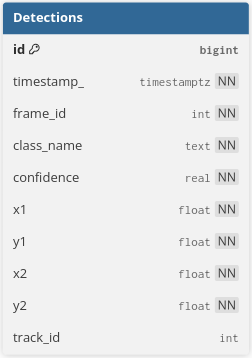
\includegraphics[width=0.3\textwidth]{images/ERD_diagram.png}
    \caption{ER diagram databázového modelu}
    \label{fig:erd}
\end{figure}

Datový model je založen na hlavní entitě \textit{detections},
která uchovává informace o jednotlivých průjezdech vozidel.
Struktura tabulky je navržena s ohledem na vysoký objem dat
a efektivní časové dotazování.


\paragraph{Popis atributů tabulky
\textit{detections}}

\begin{itemize}
    \item \textbf{id (BIGSERIAL)} – Primární klíč tabulky.
    Automaticky generovaná unikátní hodnota sloužící k jednoznačné
    identifikaci každé detekce. Typ \textit{BIGSERIAL} byl zvolen
    s ohledem na předpokládaný vysoký objem záznamů.

    \item \textbf{timestamp\_ (TIMESTAMPTZ)} – Čas detekce objektu.
    Datový typ \textit{TIMESTAMPTZ} umožňuje ukládání časové informace
    včetně časové zóny, což je důležité pro přesnou časovou analýzu
    dopravních událostí.

    \item \textbf{frame\_id (INTEGER)} – Identifikátor snímku,
    ve kterém byla detekce provedena. Umožňuje zpětné dohledání
    konkrétního frame v případě analýzy nebo ladění systému.

    \item \textbf{class\_name (TEXT)} – Název detekované třídy objektu
    (např. \textit{car}, \textit{truck}, \textit{bus}). Tento atribut
    umožňuje následnou agregaci a statistické vyhodnocení podle typu vozidla.

    \item \textbf{confidence (REAL)} – Pravděpodobnost detekce
    generovaná neuronovou sítí. Je definováno omezení
    \texttt{CHECK (confidence >= 0 AND confidence <= 1)},
    které zajišťuje validitu ukládaných hodnot.

    \item \textbf{x1, y1, x2, y2 (FLOAT)} – Souřadnice
    ohraničujícího obdélníku (bounding box) detekovaného objektu.
    Hodnoty představují levý horní a pravý dolní roh objektu
    v rámci zpracovávaného obrazu.
    Integritní omezení \texttt{CHECK (x2 > x1 AND y2 > y1)}
    zajišťuje geometrickou konzistenci dat.

    \item \textbf{track\_id (INT)} – Identifikátor sledovaného objektu,
    generovaný tracking algoritmem. Umožňuje sledování pohybu
    konkrétního vozidla napříč více snímky.
\end{itemize}

\paragraph{Indexování}

S ohledem na charakter dotazů byly vytvořeny indexy nad atributy
\textit{timestamp\_}, \textit{class\_name} a \textit{track\_id}.
Tyto indexy optimalizují zejména:

\begin{itemize}
    \item dotazy na poslední detekce,
    \item časově omezené statistiky,
    \item filtrování podle typu vozidla,
    \item analýzu pohybu konkrétního objektu.
\end{itemize}

Použití sestupného indexu nad atributem \textit{timestamp\_}
umožňuje efektivní získávání nejnovějších detekcí,
což je častý scénář v reálném provozu systému.

\subsection{Vizualizační rozhraní}
Vizualizační rozhraní systému je realizováno jako interaktivní
dashboard umožňující časovou analýzu detekcí,
agregaci podle tříd objektů a prostorovou analýzu.

\begin{figure}[H]
    \centering
    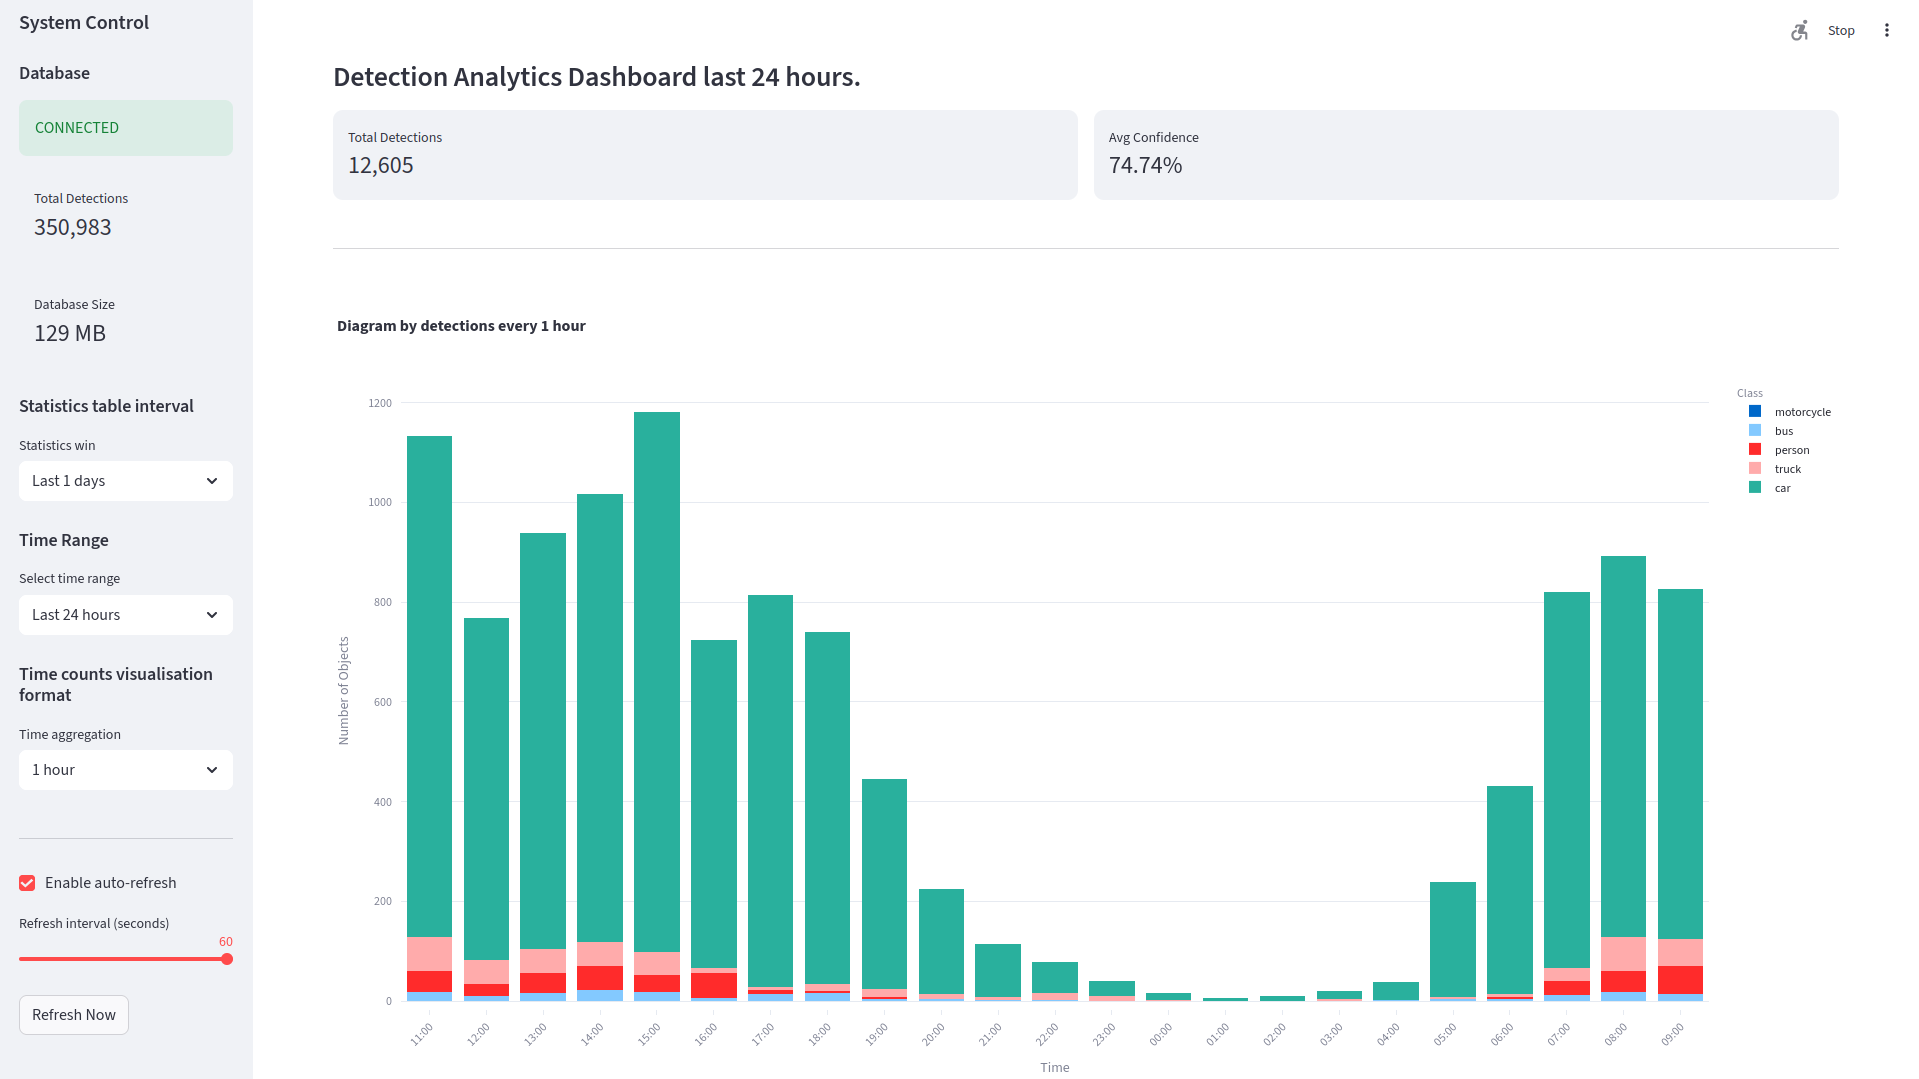
\includegraphics[width=0.95\textwidth]{images/visualisation_dashboard.png}
    \caption{Ukázka vizualizačního dashboardu systému}
    \label{fig:visualisation_dashboard}
\end{figure}

Dashboard poskytuje přehled o celkovém počtu detekcí,
průměrné hodnotě confidence a umožňuje volbu časového intervalu
pro agregaci dat.

\subsubsection{Načítání a transformace dat}
Data jsou načítána z databáze pomocí API endpointů
(\texttt{/api/detections}, \texttt{/api/statistics})
a následně transformována do datového rámce knihovny Pandas.
Součástí transformace je převod časových údajů na formát \texttt{datetime}
a rozbalení souřadnic ohraničujících obdélníků (bounding box) do samostatných
sloupců.

\subsubsection{Časová agregace detekcí}
Pro analýzu časového vývoje detekcí je využita metoda
\texttt{resample()}, která umožňuje agregaci dat
do různých časových intervalů (např. 1 minuta, 10 minut, 1 hodina).
Agregace je realizována jak globálně, tak i samostatně
pro jednotlivé třídy objektů.

\begin{lstlisting}[language=Python, caption={Časová agregace detekcí podle tříd}]
df_timeline = df.set_index("timestamp")

df_class_timeline = (
    df_timeline.groupby('class_name')
    .resample(selected_interval)
    .size()
    .reset_index(name="count")
)
\end{lstlisting}

Tento přístup umožňuje dynamickou změnu velikosti časového intervalu
a poskytuje flexibilní nástroj pro analýzu dopravní zátěže
v různých časových měřítkách.

\subsubsection{Stacked časová vizualizace}

Pro zobrazení časového vývoje detekcí podle tříd objektů
je využit stacked bar graf, který umožňuje
současné zobrazení více kategorií v rámci jednoho časového intervalu.

\begin{lstlisting}[language=Python, caption={Stacked bar graf časové agregace}]
fig = px.bar(
    df_class_timeline,
    x="timestamp",
    y="count",
    color="class_name",
    barmode="stack"
)
\end{lstlisting}

Tento typ vizualizace umožňuje identifikovat časové špičky,
porovnat relativní zastoupení jednotlivých tříd
a analyzovat změny dopravního zatížení v průběhu dne.

\chapter{Testování a vyhodnocení}
Pro vyhodnocení navrženého systému byla použita
stejná video sekvence zachycující dopravní situaci
v zimních podmínkách (sněžení).
Byla analyzována čtyřminutová část videa,
která byla zvolena jako reprezentativní
z delšího záznamu. 

Vyhodnocení bylo provedeno na dvou odlišných platformách.:

\begin{itemize}
    \item \textbf{Edge řešení (Hailo)} – detekce probíhala na zařízení
    Raspberry Pi 5 s využitím AI akcelerátoru Hailo,
    modelu YOLOv8m a sledovacího modulu \textit{hailotracker}.
    \item \textbf{GPU řešení} – detekce byla realizována
    na osobním počítači s GPU s využitím knihoven
    Ultralytics a OpenCV, modelu YOLOv11l
    a sledovacího algoritmu ByteTrack.
\end{itemize}

Detekční systém běžící na zařízení Raspberry Pi 5
je zároveň navržen jako kontinuální real-time aplikace, která nepřetržitě zpracovává video stream 
a vrací detekční události.

Získaná data jsou průběžně odesílána
prostřednictvím MQTT protokolu do backendové části systému,
kde jsou ukládána do databáze
a následně vizualizována v podobě interaktivního dashboardu.
Tento přístup umožňuje dlouhodobý sběr dat
a analýzu dopravních statistik v reálném čase.

Experimentální vyhodnocení bylo provedeno offline,
zatímco edge řešení je v praxi provozováno
v nepřetržitém režimu.

\section{Testovací scénáře}

Pro vyhodnocení navrženého systému byla použita
stejná video sekvence zachycující dopravní situaci
v zimních podmínkách (sněžení).

Video bylo analyzováno dvěma přístupy:
\begin{itemize}
    \item \textbf{Edge řešení (Hailo)} – detekce pomocí modelu YOLOv8m
    optimalizovaného pro akcelerátor Hailo a běžícího na zařízení Raspberry Pi 5.
    Pro sledování objektů byl využit modul \textit{hailotracker}
    v rámci GStreamer pipeline.

    \item \textbf{GPU řešení} – detekce pomocí modelu YOLOv11l
    realizovaná na osobním počítači s GPU,
    s využitím knihoven Ultralytics a OpenCV.
    Pro sledování objektů byl použit algoritmus ByteTrack.
\end{itemize}

Pro vyhodnocení přesnosti byla vytvořena referenční
hodnota (ground truth), která byla získána manuálním
počítáním objektů ve vybrané části video sekvence.

Pro oba přístupy byly definovány oblasti zájmu (ROI),
které se mírně lišily:

\begin{itemize}
    \item u Hailo řešení byla použita polygonální ROI,
    která byla zmenšena z důvodu omezení výskytu duplicitních detekcí,
    \item u GPU řešení byla použita obdélníková ROI,
    kde se problém ghostingu nevyskytoval v takové míře.
\end{itemize}

\section{Vyhodnocení přesnosti detekce}
Přesnost detekce byla vyhodnocena pomocí metriky accuracy.

Pro vyhodnocení detekční schopnosti byly analyzovány
výstupy obou modelů ve formě počtu detekovaných objektů
a jejich shody s referenčními hodnotami.

Výsledky pro Hailo řešení ukazují,
že bylo detekováno celkem 127 unikátních objektů
při průměrné confidence přibližně 0.77 pro třídu \textit{car}

GPU řešení detekovalo celkem 132 unikátních objektů
s průměrnou confidence přibližně 0.76 pro třídu \textit{car}


Oba modely vykazují srovnatelnou detekční přesnost,
přičemž GPU řešení dosahuje mírně vyššího počtu detekcí,
což může být způsobeno vyšší citlivostí modelu
a menším vlivem optimalizace pro edge zařízení. Jejich celková průměrná accuracy je 0.73 u GPU a 0.74 u Hailo.

\section{Vyhodnocení přesnosti sčítání}
Na základě porovnání s ručně anotovanými daty dosáhlo GPU řešení vyšší přesnosti,
zatímco Hailo řešení vykazovalo vyšší míru chyb způsobenou zejména duplicitními detekcemi (ghosting). Přesnost byla hodnocena na základě absolutní odchylky
a relativní chyby vůči ground truth.

\begin{table}[H]
\centering
\begin{tabular}{|l|c|c|c|}
\hline
\textbf{Třída} & \textbf{Hailo AI} & \textbf{GPU} & \textbf{Ruční (GT)} \\
\hline
Car & 120 & 108 & 108 \\
Bus & 4 & 11 & 3 \\
Truck & 3 & 12 & 6 \\
Person & 1 & 0 & 1 \\

\hline
\textbf{Celkem} & 127 & 132 & 118 \\
\hline
\end{tabular}
\caption{Porovnání počtu detekovaných objektů}
\end{table}

Z tabulky vyplývá,
že GPU řešení dosahuje vyšší přesnosti,
zejména u třídy \textit{Car},
kde přesně odpovídá ručnímu měření.

Naopak řešení založené na akcelerátoru Hailo
vykazuje vyšší odchylku od ground truth,
především v důsledku duplicitních detekcí
(ghosting efekt),
kdy je jeden objekt započítán vícekrát.

U tříd \textit{Bus} a \textit{Truck}
jsou patrné výraznější rozdíly mezi jednotlivými metodami,
což může být způsobeno menším počtem vzorků
a vyšší citlivostí na chybné detekce.

Celkově lze konstatovat,
že GPU řešení poskytuje přesnější výsledky,
zatímco Hailo řešení vykazuje vyšší chybu sčítání,
která je však vyvážena nižší latencí
a vyšší energetickou efektivitou.

\section{Vyhodnocení výkonnosti systému}
Výkonnost systému byla hodnocena z hlediska schopnosti real-time zpracování video streamu.

Edge řešení s využitím akcelerátoru Hailo umožňuje
spuštění detekce přímo na zařízení Raspberry Pi,
čímž odpadá nutnost přenosu dat do cloudu.

GPU řešení poskytuje vyšší flexibilitu
a přesnost detekce, avšak za cenu vyšších
hardwarových nároků.

Hlavní výhodou edge přístupu je nízká latence
a nezávislost na síťové konektivitě.

- dosažené FPS
- latence
- využití CPU
- vliv akcelerátoru

\chapter{Diskuze a prezentace výsledků}
Výsledky ukazují, že oba přístupy mají své výhody
i omezení.

Hailo řešení umožňuje efektivní real-time zpracování
na edge zařízení s nízkou spotřebou energie,
avšak může docházet k chybám způsobeným optimalizací modelu
a omezenou přesností kvantizace.

GPU řešení dosahuje vyšší přesnosti detekce
a stabilnějšího sledování objektů,
zejména díky použití pokročilejšího modelu
a robustnějšího tracking algoritmu.

Rozdíly v přesnosti byly také ovlivněny
rozdílnou definicí ROI oblastí,
kde menší polygonální oblast u Hailo řešení
byla zvolena za účelem redukce chyb způsobených ghostingem.

\chapter{Závěr}
- Shrnutí dosažených cílů.
- Zhodnocení přínosu a praktické využitelnosti práce.
- Návrhy na další rozšíření a vylepšení.

\sloppy
\printbibliography[title=Seznam použitých zdrojů]
\cite{hailo_alpr_2024}
\cite{harris_numpy_2020}
\cite{hyndman_forecasting_2018}
\cite{li_edge_ai_2020}
\cite{johansson_numerical_python_2019}
\cite{mckinney_pandas_2010}
\cite{mqtt_oasis_2019}
\cite{plotly_docs_2015}
\cite{psycopg_docs_2025}
\cite{python_docs_313_2025}
\cite{raspberrypi_ai_kit}
\cite{raspberrypi_docs_2024}
\cite{redmon_yolo_2016}
\cite{szeliski_computer_vision}
\cite{zhou_traffic_survey_2024}

\appendix

\chapter{Externí přílohy\label{sec:ep}}

V této kapitole stačí uvést pouze základní strukturu úložiště (co se kde nalézá a jakou má funkci) například v podobě tabulky. 

\begin{longtable}{ll}
\hline
ki-thesis.pdf & text práce v PDF \\
ki-thesis.tex & zdrojový kód práce v \LaTeX{}u \\
kitheses.cls & definice třídy dokumentů (rozšířená třída \texttt{scrbook} \\
thesis.bib & bibliografická databáze (exportována z citace.com) \\
LOGO\_PRF\_CZ\_RGB\_standard.jpg  & logo fakulty s českým textem \\
LOGO\_PRF\_EM\_RGB\_standard.jpg  & logo fakulty s anglickým textem  \\
\hline
\end{longtable}

Všechny tyto soubory jsou potřeba pro překlad dokumentu (logo stačí jedno v příslušné jazykové verzi).


\end{document}

